%!TEX root=../../main.tex

%\begin{doublespace}
\begin{spacing}{1.5}

\chapter{Foundations for inference}
\label{foundationsForInference}

\begin{comment}
Issues pending

-- Remove the poker example in the clt section.


-- Missing section on using confidence intervals for tests.

	
\end{comment}


On average, how many days a week are high school students physically active? How many hours of sleep per night do they get? In theory, one way to answer these questions about the youth population in the United States is to collect information from all 21.2 million high-school aged youth in the country -- however, this strategy is simply impossible. Instead, a representative sample of students can be selected for study, and the information from the sample used to learn about the population. In statistical terms, a characteristic of a population, such as the average amount of sleep per night for high-school aged students, is called a \term{population parameter}. When carried out correctly, sampling from a population is an efficient way to estimate a population parameter. Drawing inferences about the characteristics of a population from a sample represents a primary goal of statistics. This chapter introduces the important ideas in drawing estimates from samples by discussing methods of inference for a population mean, $\mu$. 

This chapter also discusses three widely used tools in statistics: point estimates (single number estimates) for a population mean, interval estimates that include both a point estimate and a margin of error, and a method for testing scientific hypotheses about $\mu$. The concepts used in this chapter will appear throughout the rest of the book. While particular equations or formulas may change to reflect the details of a problem at hand, the fundamental ideas will not. 

\index{data!yrbss|(}

The United States Centers for Disease Control and Prevention (CDC) lists one of their roles as "promoting healthy and safe behaviors, communities, and environment."\footnote{\url{http://www.cdc.gov/about/organization/mission.htm}} The first step in health promotion is understanding health behaviors; the CDC periodically conducts several surveys, including the Youth Risk Behavior Surveillance System (YRBSS).\footnote{\url{http://www.cdc.gov/healthyyouth/data/yrbs/index.htm}} Between 1991 and 2013, 2.6 million high school students have participated in more than 1,100 separate surveys. The next few sections discuss the dataset \data{yrbss}, which contains the responses of the 13,583 high school students who participated in the 2013 YRBSS.\footnote{\oiRedirect{textbook-yrbss}{www.cdc.gov/healthyyouth/data/yrbs/data.htm}} Part of this dataset is shown in Table~\ref{yrbssDF}, with the variables described in Table~\ref{yrbssVariables}.

\begin{table}[h]
\centering
\begin{tabular}{rrllrrlrr}
  \hline
ID & age & gender & grade & height & weight & helmet & active & lifting \\ 
  \hline
1 &  14 & female & 9 &  &  & never &   4 &   0 \\ 
  2 &  14 & female & 9 &  &  & never &   2 &   0 \\ 
  3 &  15 & female & 9 & 1.73 & 84.37 & never &   7 &   0 \\ 
  $\vdots$ & $\vdots$ & $\vdots$ & $\vdots$ & $\vdots$ & $\vdots$ & $\vdots$ & $\vdots$ & $\vdots$ \\
  13582 &  17 & female & 12 & 1.60 & 77.11 & sometimes &   5 &  \\ 
  13583 &  17 & female & 12 & 1.57 & 52.16 & did not ride &   5 &  \\ 
  \hline
\end{tabular}
\caption{Five cases from the \data{yrbss} dataset. Blank observations represent missing data. For example, the height and weight of students 1 and 2 are missing\textC{\vspace{-2mm}}}
\label{yrbssDF}
\end{table}
% library(openintro); library(xtable); data(yrbss); xtable(rbind(head(yrbss, 4), tail(yrbss, 2))[, c("age", "gender", "grade", "height", "weight", "helmet_12m", "physically_active_7d", "strength_training_7d")])

\begin{table}[h]
\centering\small
\begin{tabular}{l p{110mm}}
\hline
{\bf age} & {\bf Age of the student.} \\
\hline
\var{gender} & {Sex of the student.} \\
\var{grade} & Grade in high school (9-12) \\
\var{height} & Height, in meters. (1 m = ~3.28 ft) \\
\var{weight} & Weight, in kilograms (1 kg = ~2.2 lbs) \\
\var{helmet} & Frequency that the student wore a helmet while biking in the last 12~months. \\
\var{active} & Number of days physically active for 60+ minutes in the last 7 days. \\
\var{lifting} & Number of days of strength training (e.g. lifting weights) in the last 7 days. \\
\hline
\end{tabular}
\caption{Variables and their descriptions for the \data{yrbss} data set.}
\label{yrbssVariables}
\end{table}

\index{data!yrbss.samp|(}

CDC public health scientists used the responses of 13,572 students to estimate the health behaviors of a \term{target population}: the approximately 21.2 million high school aged students in the US population in 2013. 

This chapter illustrates inference for a population mean by treating the CDC sample of 13,582 students as an artificial target population. A random sample of 100 participants can then be used to estimate health behaviors for the "target population" of 13,572 respondents. In other words, this chapter demonstrates methods for estimating the behaviors for 13,572 students using only the information from a sample of 100 students. 

While the individuals in \data{yrbss} are not truly a target population, treating them as such allows for the estimates obtained by inference to be checked against the "population parameters" of \data{yrbss} -- not possible in a realistic setting, since population parameters (such as the average hours of sleep per night across 21.2 million students) are typically unknown.\footnote{Hence, the need for inference!}

The dataset \data{yrbss.samp} contains the data for 100 student responses randomly sampled from the larger \data{yrbss} dataset (Table~\ref{yrbssSampDF}).\footnote{About 10\% of high schoolers for each variable chose not to answer the question. Multiple regression (see Chapter~\ref{multipleAndLogisticRegression}) was used to predict what those responses would have been. For simplicity, we will assume that these predicted values can be used for the unknown responses.} Histograms summarizing the \var{height}, \var{weight}, \var{active}, and \var{lifting} variables from \data{yrbss.samp} are shown in Figure~\ref{yrbssSampHistograms}.

\begin{table}
	\centering
	\begin{tabular}{rrllrrlrr}
		\hline
		ID & age & gender & grade & height & weight & helmet & active & lifting \\ 
		\hline
		5653 &  16 & female & 11 & 1.50 & 52.62 & never &   0 &   0 \\ 
		9437 &  17 & male & 11 & 1.78 & 74.84 & rarely &   7 &   5 \\ 
		2021 &  17 & male & 11 & 1.75 & 106.60 & never &   7 &   0 \\ 
		$\vdots$ & $\vdots$ & $\vdots$ & $\vdots$ & $\vdots$ & $\vdots$ & $\vdots$ & $\vdots$ & $\vdots$ \\
		2325 &  14 & male & 9 & 1.70 & 55.79 & never &   1 &   0 \\ 
		\hline
	\end{tabular}
	\caption{Four observations for the \data{yrbss.samp} data set, which represents a simple random sample of 100 high schoolers from the 2013 YRBSS.}
	\label{yrbssSampDF}
	% library(openintro); library(xtable); data(yrbss); xtable(rbind(head(yrbss.samp, 3), tail(yrbss.samp, 1))[, c("age", "gender", "grade", "height", "weight", "helmet_12m", "physically_active_7d", "strength_training_7d")])
	%library(openintro); library(xtable); data(yrbss); data(yrbss.samp); xtable(yrbss.amp[c(1,2,3,100),])
\end{table}

% WARNING: This figure is referenced in Section 4.2
\begin{figure}
\centering
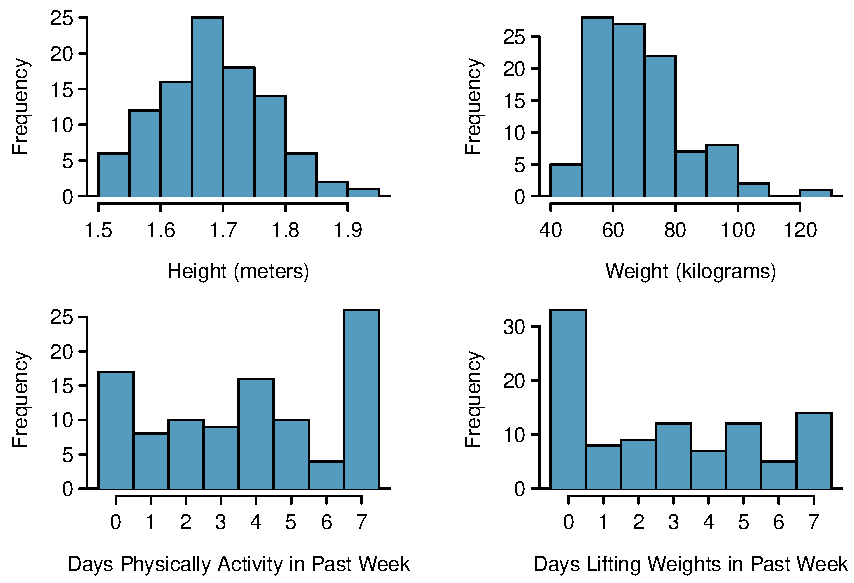
\includegraphics[width=0.8\textwidth]
{ch_inference_foundations_oi_biostat/figures/yrbssSampHistograms/yrbssSampHistograms} 
\caption{Histograms of \var{height}, \var{weight}, \var{activity}, and \var{lifting} for the sample data (\data{yrbss.samp}).}
\label{yrbssSampHistograms}
\end{figure}

\newpage

%__________________
\section[Variability in estimates]{Variability in estimates} %\sectionvideohref{youtube-DNIauUrRIEM&list=PLkIselvEzpM7Pjo94m1e7J5jkIZkbQAl4}}
\label{variabilityInEstimates}

\index{point estimate|(}

Summary statistics calculated using the \data{yrbss.samp} data can be used to estimate features of the 13,582 high school students in \data{yrbss}. For example, the average number of days active per week of the students in \data{yrbss.samp} is:

\begin{align*}
\overline{x}_{active} &= \frac{0 + 7 + \dots + 1}{100} = 3.75.
\end{align*}
%library(openintro); data(yrbss.samp); d <- yrbss.samp$physically_active_7d; mean(d); d

The sample mean $\overline{x} = 3.75$ days per week is a \term{point estimate} of the population mean. Sample means are the natural choice of summary statistic for estimating a population mean. If a second random sample of 100 were taken, the new sample mean would likely be different as a result of \term{sampling variation}. While estimates generally vary from one sample to another, the population mean is a fixed value: the average number of days active per week for all 13,582 students in \data{yrbss}.

Other population parameters, such as population median or population standard deviation, are also estimated using sample versions. Table~\ref{ptEstimatesYrbssActive} shows estimates of the population mean, median, and standard deviation for respondents in \data{yrbss}, using \data{yrbss.samp}, as well as the "population parameters" calculated by using the full \data{yrbss} dataset. The estimates differ slightly from the population parameters, but not by much -- in fact, the estimate for median is equal to the population median.

\begin{table}[h]
	\centering
	\begin{tabular}{ l rr}
		\hline
		\var{active}	& estimate & parameter  \\
		\hline
		mean		& 3.75 & 3.90 \\
		median		& 4.00 & 4.00 \\
		st. dev.		& 2.556 & 2.564 \\
		\hline
	\end{tabular}
	\caption{Point estimates and parameter values for the \var{active} variable. The parameters were obtained by computing the mean, median, and SD for all respondents (i.e. the complete set of responses in \data{yrbss}).}
	\label{ptEstimatesYrbssActive}
\end{table}

\begin{comment}

%JV: material with other summary stats

The \data{yrbss.samp} data can be used to estimate four features of the 13,582 high school students in \data{yrbss}: 1) average height (in meters), 2) average weight, 3) average number of days per week physically active (for more than 60 minutes at a time), 4) average body mass index (BMI).

Sample means are the natural choice of summary statistic for estimating a population mean. The average height of the students in \data{yrbss.samp} is:

\begin{align*}
\overline{x}_{\text{height}} = \frac{1.50 + 1.78 + \dots + 1.70}{100} = 1.697.
\end{align*}
%library(openintro); data(yrbss.samp); mean(yrbss.samp$height); yrbss.samp$height

The sample mean $\overline{x} = 1.697$ meters (5 feet, 6.8 inches) is a \term{point estimate} of the population mean. If a second random sample of 100 were taken, the new sample mean would likely be different as a result of \term{sampling variation}.  Estimates generally vary from one sample to another, whereas the population mean is a fixed value; thus, the distinction between a sample mean versus a population mean is important. 

The sample means of \var{weight} and \var{active} provide estimates of the average weight and number of days active per week of YRBSS respondents. On average, students weigh 68.89 kilograms (about 151.6 pounds) and are active 3.75 days per week:
\begin{align*}
\overline{x}_{weight} &= \frac{52.6 + 74.8 + \dots + 55.8}{100} = 68.89
&\overline{x}_{active} &= \frac{0 + 7 + \dots + 1}{100} = 3.75.
\end{align*}
%library(openintro); data(yrbss.samp); d <- yrbss.samp$weight; mean(d); d
%library(openintro); data(yrbss.samp); d <- yrbss.samp$physically_active_7d; mean(d); d

BMI is used by health professionals to gauge whether an individual's weight is consistent with their height. While BMI is not one of the variables in the dataset, it can be calculated from height and weight (measured in metric units) with the formula:

\[ \text{bmi} = \frac{\text{weight}}{\text{height}{^2}}\]

For example, the respondent with ID 5553 has BMI of 23.39 ($52.62/1.5^{2}$). Larger values of BMI indicate higher levels of body fat. Average BMI in \data{yrbss.samp} is found by calculating BMI values for each respondent, then computing the average of the BMI values. Average BMI in \data{yrbss.samp} is 23.92. Since adolescent size and body type can change with age, there are no population norms for BMI in the age range of YRBSS respondents as there are for adults.  For an adult, a BMI of 23.4 would be considered within the range of normal weight, neither under- nor over-weight.

%%%  note that bmi cutpoints for children and teens are not the same as for adults. The CDC does not seem to recommend levels for health bmi for teens

Other population parameters, such as population median or population standard deviation, are also estimated using sample versions. Table~\ref{ptEstimatesYrbssActive} shows estimates of the population mean, median, and standard deviation for respondents in \data{yrbss}, using \data{yrbss.samp}, as well as the "population parameters" calculated by using the full \data{yrbss} dataset. The estimates differ slightly from the population parameters, but not by much -- in fact, the estimate for median is equal to the population median. Note that the estimates will vary based on the sample taken; these estimates are specific to the data in \data{yrbss.samp}.

\begin{table}[h]
\centering
\begin{tabular}{ l rr}
\hline
\var{active}	& estimate & parameter  \\
\hline
mean		& 3.75 & 3.90 \\
median		& 4.00 & 4.00 \\
st. dev.		& 2.556 & 2.564 \\
\hline
\end{tabular}
\caption{Point estimates and parameter values for the \var{active} variable. The parameters were obtained by computing the mean, median, and SD for all respondents (i.e. the complete set of responses in \data{yrbss}).}
\label{ptEstimatesYrbssActive}
\end{table}

\end{comment}

\begin{exercise} \label{peOfDiffActiveBetweenGender}
	How would one estimate the difference in days active for men and women? If $\overline{x}_{\text{men}} = 4.3$ and $\overline{x}_{\text{women}} = 3.2$, then what is a good point estimate for the population difference?\footnote{If $\overline{x}_{\text{men}} = 4.3$ and $\overline{x}_{\text{women}} = 3.2$, the difference of the two sample means, $4.3 - 3.2 = 1.1$, would be an estimate of the difference. In other words, it can be concluded from the sample that on average, the male respondents are physically active about 1.1 days per week more than the female respondents.}
\end{exercise}
%library(openintro); library(xtable); data(yrbss); data(yrbss.samp); (x <- by(yrbss.samp$physically_active_7d, yrbss.samp$gender, mean)); diff(x)

While point estimates rarely equal population parameters (the median in Table~\ref{ptEstimatesYrbssActive} is one of those rare examples), they do become more accurate as more data become available. The running mean from the variable \var{active} in \data{yrbss.samp}, shown in Figure~\ref{yrbssActiveRunningMean}, demonstrates this principle. A \term{running mean} is a sequence of sample means in which sample size increases by 1 for each mean that is calculated. For example, the second mean in the sequence is the average of the first two observations, and the third mean in the sequence is the average of the first three observations. 

\begin{figure}[h]
	\centering
	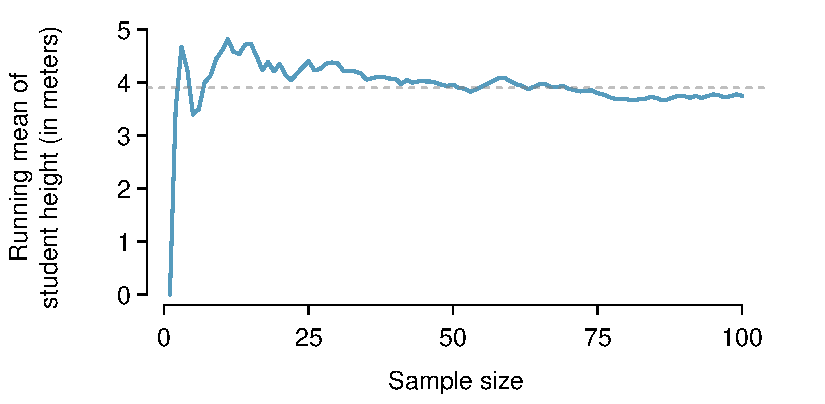
\includegraphics[width=0.72\textwidth]{ch_inference_foundations_oi_biostat/figures/yrbssActiveRunningMean/yrbssActiveRunningMean}
	\caption{The mean computed after gradually adding each individual to the sample (data from \data{yrbss.samp}). The mean tends to approach the true population mean as sample size increases. Running means calculated from a different random sample from \data{yrbss} would also show the same behavior.}
	\label{yrbssActiveRunningMean}
\end{figure}

As the sample size increases, the running mean approaches the population mean of 3.90 days. Thus, the CDC officials can be reasonably confident that means calculated using data from 13,582 students provide an accurate estimate of the population mean for the 21.2 million students.  Section~\ref{seOfTheMean} provides formulas for calculating how accurate sample estimates are likely to be.

\subsection{The sampling distribution for the mean}

The sample mean calculated from \data{yrbss.samp} was 3.75 days active per week. Another random sample of 100 participants might produce a different value of $\overline{x}$, such as 3.22 days; repeated random sampling would result in additional different values, perhaps 3.67 days, 4.10 days, and so on. Each sample mean can be thought of as a single observation from a random variable $\overline{X}$. The distribution of $\overline{X}$ is referred to as the \term{sampling distribution of the sample mean}, and has its own mean and standard deviation like the random variables discussed in Chapter 3. The concept of a sampling distribution can be illustrated by taking repeated random samples from \data{yrbss}, the artificial target population. Figure~\ref{yrbssActive1000SampDist} shows a histogram of sample means from 1,000 random samples of size 100 from \data{yrbss}. The histogram provides a close approximation of the theoretical sampling distribution of $\overline{X}$ for sample sizes of 100. 

\begin{figure}[h]
	\centering
	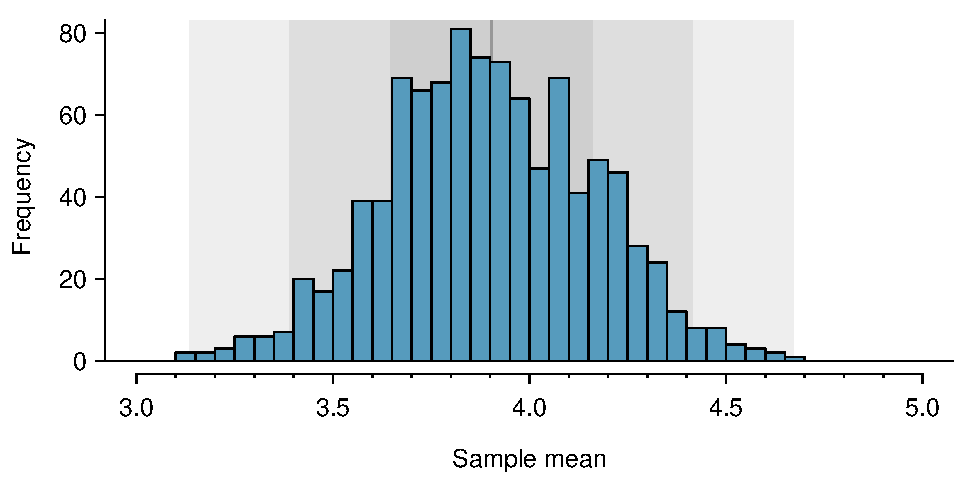
\includegraphics[width=0.9\textwidth]
	{ch_inference_foundations_oi_biostat/figures/yrbssActive1000SampDist/yrbssActive1000SampDist}
	\caption{A histogram of 1000 sample means for number of days physically active per week, where the samples are of size $n=100$.}
	\label{yrbssActive1000SampDist}
\end{figure}

\begin{termBox}{\tBoxTitle{Sampling distribution}
The sampling distribution is the distribution of the point estimates based on samples of a fixed size from a certain population. It is useful to think of a particular point estimate as being drawn from a sampling distribution.}
\end{termBox}

Since the complete sampling distribution consists of means for all possible samples of size 100, drawing a much larger number of samples would provide a more accurate view of the distribution; the left panel of Figure~\ref{yrbssActiveBigSampDist} shows the distribution calculated from 100,000 sample means. 
 
\begin{figure}[hht]
 	\centering
 	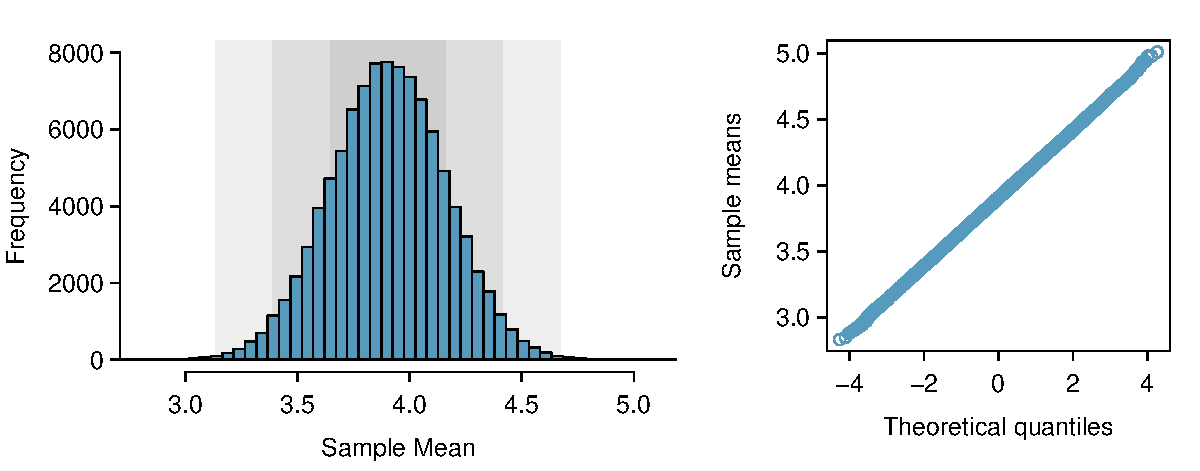
\includegraphics[width=\textwidth]
 	{ch_inference_foundations_oi_biostat/figures/yrbssActiveBigSampDist/yrbssActiveBigSampDist}
 	\caption{The left panel shows a histogram of the sample means for 100,000 random samples. The right panel shows a normal probability plot of those sample means.}
 	\label{yrbssActiveBigSampDist}
\end{figure}
 
 A normal probability plot of these sample means is shown in the right panel of Figure~\ref{yrbssActiveBigSampDist}. All of the points closely fall around a straight line, implying that the distribution of sample means is nearly normal (see Section~\ref{normalDist}). This result follows from the Central Limit Theorem.
 
 \begin{termBox}{\tBoxTitle{Central Limit Theorem, informal description}
 		If a sample consists of at least 30 independent observations and the data are not strongly skewed, then the distribution of the sample mean is well approximated by a~normal model.\index{Central Limit Theorem}}
 \end{termBox}

\subsection{Standard error of the mean}
\label{seOfTheMean}

The sampling distribution for the mean shown in Figures~\ref{yrbssActive1000SampDist} and \ref{yrbssActiveBigSampDist} is unimodal and symmetric. The center of the histogram is approximately the mean of the random variable $\overline{X}$. Statistical theory can be used to show that the mean of the sampling distribution for $\overline{X}$ is exactly equal to the population mean $\mu$.

However, in almost any study, conclusions about a population parameter must be drawn from the data collected from a single sample. The sampling distribution of $\overline{X}$ is a theoretical concept, since obtaining repeated samples by conducting the studies many times is not possible. In other words, it is not feasible to calculate the population mean $\mu$ through finding the mean of the sampling distribution for $\overline{X}$.

The conceptual link between a sample mean and the sampling distribution of $\overline{X}$ is valuable in that it allows for the \term{standard error} of the sample mean to be calculated. The standard error of the sample mean measures the sample-to-sample variability of $\overline{X}$, the extent to which values of the repeated sample means oscillate around the population mean. 

The standard error of the sample mean is calculated by dividing the population standard deviation ($\sigma_{x}$) by the square root of the sample size $n$. Since the population standard deviation $\sigma$ is typically unknown, the sample standard deviation $s$ can be used as a reasonably good estimate of $\sigma$. If $\overline{x}$ is the sample mean of days per week active,

\[\text{SE}_{\overline{x}} = \dfrac{\sigma_{x}}{\sqrt{n}} = \dfrac{2.60}{\sqrt{100}} = 0.260;  \qquad \text{SE}_{\overline{x}} \approx \dfrac{s_{x}}{\sqrt{n}} = \dfrac{2.556}{\sqrt{100}} = 0.256.\]

This estimate tends to be sufficiently good when the sample size is at least 30 and the population distribution is not strongly skewed. In the case of skewed distributions, a larger sample size is necessary.

The probability tools of Section~\ref{randomVariablesSection} can be used to derive the formula $\sigma_{\overline{X}} = \sigma_x/\sqrt{n}$, but the derivation is not shown here. Conceptually, larger sample sizes result in sampling distributions that have decreasing variability. Increasing sample size causes $\overline{X}$ to be clustered more tightly around the population mean $\mu$, allowing for more accurate estimates of $\mu$ from a single sample.

Note that the standard error of the sample mean can be approximated by the standard deviation of $\overline{X}$, but that this method of estimating the standard error is not possible when there is only a single sample. The sample provides only one observation from $\overline{X}$ and cannot provide any information about the variability of the sampling distribution.

% \term{standard error (SE)}\index{SE}\marginpar[\raggedright\vspace{-4mm}

% $SE$\\\footnotesize standard\\error]{\raggedright\vspace{-4mm}

% $SE$\\\footnotesize standard\\error} of the estimate.

\begin{termBox}{\tBoxTitle{The standard error (SE) of the sample mean}
		Given $n$ independent observations from a population with standard deviation $\sigma$, the standard error of the sample mean is equal to \vspace{-1mm}
		\begin{align*}
		\text{SE} = \frac{\sigma}{\sqrt{n}}.
		\label{seOfXBar}
		\end{align*}\vspace{-3mm}%
		
		When the sample size is at least 30 and the population distribution is not strongly skewed, the standard error of the sample mean can be estimated by using the sample standard deviation $s$ as an estimate of $\sigma$.
	}
\end{termBox}


\begin{comment}

%JV: edited this summary, hidden for now because it doesn't seem as necessary with the shortened section

\begin{termBox}{\tBoxTitle{Point estimate terminology: summary}
\begin{itemize}
	\setlength{\itemsep}{0mm}	
	\item The population parameters $\mu$ and $\sigma$ are characteristics of the target population from which a sample is drawn. 
	
	\item Within a sample, the sample mean is denoted by $\overline{x}$ and the sample standard deviation is denoted by $s$. 
	
	\item The distribution of the random variable $\overline{X}$ is the collection of sample means if multiple samples were repeatedly drawn from a population. The distribution of $\overline{X}$ has its own mean $\mu_{\overline{X}}$ and standard deviation $\sigma_{\overline{X}}$. 
	
	\item With random sampling, the mean of the random variable $\overline{X}$ is always equal to the population mean $\mu$.  In the notation of Chapter 3, $\mu_{\overline{X}} = E(\overline{X}) = \mu$.
	
	\item  The standard deviation of $\overline{X}$, written $\sigma_{\overline{X}}$, is called its standard error (SE). 
	
	\item The standard error of the sample mean, as calculated from a single sample of size $n$, is equal to $\dfrac{\sigma}{\sqrt{n}}$. The standard error is abbreviated by SE and is usually estimated by using $s$, such that $SE = \dfrac{s}{\sqrt{n}}$.
	
\end{itemize}
		
	}
\end{termBox}

\end{comment}

\index{point estimate|)}

\begin{comment}

%JV: older version of summary

The terminology for point estimates can be confusing, and is worth restating:  

\begin{itemize}
\setlength{\itemsep}{0mm}	
	\item The population parameters $\mu$ and $\sigma$ are characteristics of the target population from which a sample is drawn. 
	
	\item In a single sample, the arithmetic average of the values in the sample (the sample mean) is denoted by $\overline{x}$. The sample standard deviation is denoted by $s$. 
	
	\item If repeated samples could be taken, the distribution of the random variable $\overline{X}$ is the collection of sample means (one for each sample). The distribution of $\overline{X}$ is called its sampling distribution, which itself has a mean $\mu_{\overline{X}}$ and standard deviation $\sigma_{\overline{X}}$. 
	
	\item With random sampling, the mean of the random variable $\overline{X}$ is always equal to the population mean $\mu$.  In the notation of Chapter 3, $\mu_{\overline{X}} = E(\overline{X}) = \mu$.
	
	\item  The standard deviation of $\overline{X}$, written $\sigma_{\overline{X}}$, is called its standard error (SE). 
	
	\item The standard error of the sample mean, as calculated from a single sample of size $n$, is equal to $\dfrac{\sigma}{\sqrt{n}}$. The standard error is abbreviated by SE and is usually estimated by using $s$, such that $SE = \dfrac{s}{\sqrt{n}}$.
	
\end{itemize}

\index{point estimate|)}

\end{comment}

\section[Confidence intervals]{Confidence intervals} %\sectionvideohref{youtube-FUaXoKdCre4&list=PLkIselvEzpM7Pjo94m1e7J5jkIZkbQAl4}}
\label{confidenceIntervals}
\subsection{Interval estimates for a population parameter}

While a point estimate consists of a single value, an interval estimate gives a plausible range of values for a parameter. When estimating a population mean $\mu$, a \term{confidence interval} for $\mu$ has the general form

\[(\overline{x} -m, \ \overline{x} + m) = \overline{x} \pm m, \]
where $m$ is the margin of error. Intervals that have this form are called \term{two-sided confidence intervals} because they provide both lower and upper bounds, $\overline{x} - m$ and $\overline{x} + m$, respectively. One-sided sided intervals are discussed in Section~\ref{onesidedCIs}.

The standard error of the sample mean is the standard deviation of its distribution; additionally, the distribution of sample means is nearly normal. Thus, under the normal model, the sample mean $\overline{x}$ will be within 1.96 standard errors of the population mean $\mu$ approximately 95\% of the time.\footnote{In other words, the $Z$-score of 1.96 is associated with 2.5\% area to the right (and $Z$ = -1.96 has 2.5\% area to the left); this can be found on normal probability tables or from using statistical software.} If an interval is constructed that spans 1.96 standard errors from the point estimate in either direction, a data analyst can be 95\% \term{confident} that the population mean is somewhere within the interval

\begin{align}
\text{point estimate}\ \pm\ 1.96\times \text{SE}, 
\label{95PercentCIWhenUsingNormalModel}
\end{align}

The value 95\% is an approximation, accurate when the sampling distribution for the sample mean is close to that of a normal distribution. This assumption holds when the sample size is sufficiently large (guidelines for `sufficiently large' are given in Section~\ref{ch4Summary}).

The phrase "95\% confident" has a subtle interpretation: if many samples were drawn from a population, with each one used to calculate a confidence interval using Equation~\ref{95PercentCIWhenUsingNormalModel}, about 95\% of those intervals would contain the population mean $\mu$. Figure~\ref{95PercentConfidenceInterval} illustrates this process with 25 samples taken from \data{yrbss}. Twenty-four of the resulting confidence intervals contain the population average number of days per week that respondents are physically active, $\mu$ = 3.90 days, while one does not. 

Just as with the sampling distribution of the sample mean, the interpretation of a confidence interval relies on the abstract construct of repeated sampling. A data analyst, who can only observe one sample, does not know whether the population mean lies within the single interval calculated. The uncertainty is due to random sampling -- by chance, it is possible to select a sample from the population that has unusually high (or low) values, resulting in a sample mean $\overline{x}$ that is relatively far from $\mu$, and by extension, a confidence interval that does not contain $\mu$. 

\begin{figure}[hht]
   \centering
   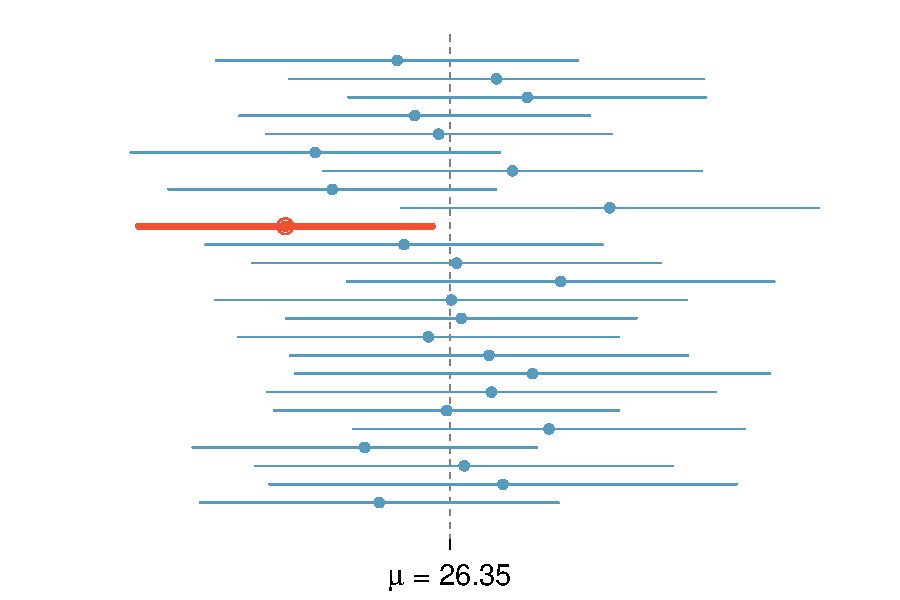
\includegraphics[width=0.78\textwidth]
{ch_inference_foundations_oi_biostat/figures/95PercentConfidenceInterval/95PercentConfidenceInterval}
   \caption{Twenty-five samples of size $n=100$ were taken from \data{yrbss}. For~each sample, a confidence interval was created to try to capture the average number of days per week that students are physically active. Only~1 of these~25 intervals did not capture the true mean, $\mu = 3.90$~days.}
   \label{95PercentConfidenceInterval}
\end{figure}

\begin{comment}

\begin{exercise}
In Figure~\ref{95PercentConfidenceInterval}, one interval does not contain 3.90 minutes. Does this imply that the mean cannot be 3.90?\footnote{Just as some observations occur more than 2 standard deviations from the mean, some point estimates will be more than 2 standard errors from the parameter. A confidence interval only provides a plausible range of values for a parameter. While we might say other values are implausible based on the data, this does not mean they are impossible.}
\end{exercise}

\end{comment}

\begin{example}{The sample mean of days active per week from \data{yrbss.samp} is 3.75~days. The standard error, as estimated using the sample standard deviation, is $\text{SE}=\frac{2.564}{\sqrt{100}} = 0.2564$~days. Calculate an approximate 95\% confidence interval for the average days active per week for all YRBSS students.}
Using Equation~\ref{95PercentCIWhenUsingNormalModel}:
\[3.75\ \pm\ 1.96 \times  0.26 \quad \rightarrow \quad (3.24, 4.26)\]
Based on these data, we can be about 95\% confident that the average days active per week for all YRBSS students was larger than 3.24 but less than 4.26~days. The interval extends out 1.96 standard errors from the point estimate, $\overline{x}_{\text{active}}$.
\end{example}
% library(openintro); library(xtable); d <- yrbss.samp; mean(d$physically_active_7d); sd(d$physically_active_7d); sd(yrbss$physically_active_7d, na.rm=TRUE)

\begin{exercise} \label{95CIExerciseForAgeOfYrbssSamp1}
The sample data suggest that the average YRBSS student height is $\overline{x}_{\text{height}} = 1.697$ meters with a standard error of 0.0088 meters (estimated using the sample standard deviation, 0.088 meters). What is an approximate 95\% confidence interval for the average height of all of the YRBSS students?\footnote{Apply Equation~\ref{95PercentCIWhenUsingNormalModel}: $1.697 \ \pm \ 2\times 0.0088 \rightarrow (1.6798, 1.7142)$.  We are about 95\% confident the average height of all YRBSS students was between 1.6798 and 1.7142 meters (5.5~to 5.6~feet).}
\end{exercise}
% library(openintro); d <- yrbss.samp; mean(d$height); sd(d$height)

\begin{comment}

\subsection{The sampling distribution for the mean}

%JV: moved to 4.1

 Figure~\ref{yrbssActive1000SampDist} showed an approximation of the distribution of sample means for the variable \data{active} calculated from 1,000 random samples of size $n= 100$. Since the complete sampling distribution consists of means for all possible samples of size 100, drawing a much larger number of samples would provide a more accurate view of the distribution; the left panel of Figure~\ref{yrbssActiveBigSampDist} shows the distribution calculated from 100,000 sample means. 

\begin{figure}[hht]
   \centering
   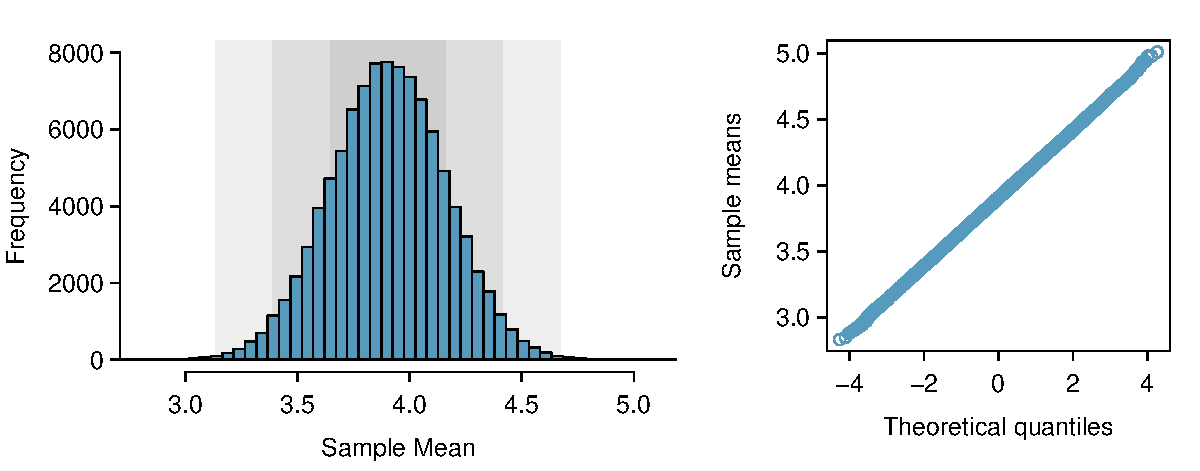
\includegraphics[width=\textwidth]
{ch_inference_foundations_oi_biostat/figures/yrbssActiveBigSampDist/yrbssActiveBigSampDist}
   \caption{The left panel shows a histogram of the sample means for 100,000 random samples. The right panel shows a normal probability plot of those sample means.}
   \label{yrbssActiveBigSampDist}
\end{figure}

A normal probability plot of these sample means is shown in the right panel of Figure~\ref{yrbssActiveBigSampDist}. All of the points closely fall around a straight line, implying that the distribution of sample means is nearly normal (see Section~\ref{normalDist}). This result is due to by the Central Limit Theorem, summarized here and covered in more detail in Section~\ref{cltSection}.

\begin{termBox}{\tBoxTitle{Central Limit Theorem, informal description}
If a sample consists of at least 30 independent observations and the data are not strongly skewed, then the distribution of the sample mean is well approximated by a~normal model.\index{Central Limit Theorem}}
\end{termBox}

The choice of 2 standard errors in Equation~\ref{95PercentConfidenceIntervalFormula} was based on the general guideline that roughly 95\% of the time, observations are within two standard deviations of the mean. Under the normal model, this can be made more accurate by using 1.96 in place~of~2.
\begin{align}
\text{point estimate}\ \pm\ 1.96\times \text{SE}
\label{95PercentCIWhenUsingNormalModel}
\end{align}
% If a point estimate, such as $\overline{x}$, is associated with a normal model and standard error $SE$, then we use this more precise 95\% confidence interval.

The Central Limit Theorem is discussed in more detail in Section~\ref{cltSection}.

\end{comment}

\subsection{Changing the confidence level}
\label{changingTheConfidenceLevelSection}

\index{confidence interval!confidence level|(}

Ninety-five percent confidence intervals are the most commonly used interval estimates, but intervals with confidence levels other than 95\% can also be constructed. The general formula for a confidence interval (for the population mean $\mu$) is given by 
\begin{align}
	\overline{x} \pm \ z^{\star} \times \text{SE},
\end{align}
where $z^{\star}$ is chosen according to the confidence level. When calculating a 95\% confidence level, $z^{\star}$ is 1.96, since the area within 1.96 standard deviations of the mean captures 95\% of the distribution.

To construct a 99\% confidence interval, $z^{\star}$ must be chosen such that 99\% of the normal curve is captured between -$z^{\star}$ and $z^{\star}$.

\begin{example}{Let $Y$ be a normally distributed random variable. Ninety-nine percent of the time, $Y$ will be within how many standard deviations of the mean?}
	This is equivalent to the $z$-score with 0.005 area to the right of $z$ and 0.005 to the left of $-z$. In the normal probability table, this is the $z$-value that with .005 area to its right and .995 area to its left. The closest two values are 2.57 and 2.58; for convenience, round up to 2.58. The unobserved random variable $Y$ will be within 2.58 standard deviations of $\mu$ 99\% of the time, as shown in Figure~\ref{choosingZForCI}.
\end{example}

\begin{figure}[h]
	\centering
	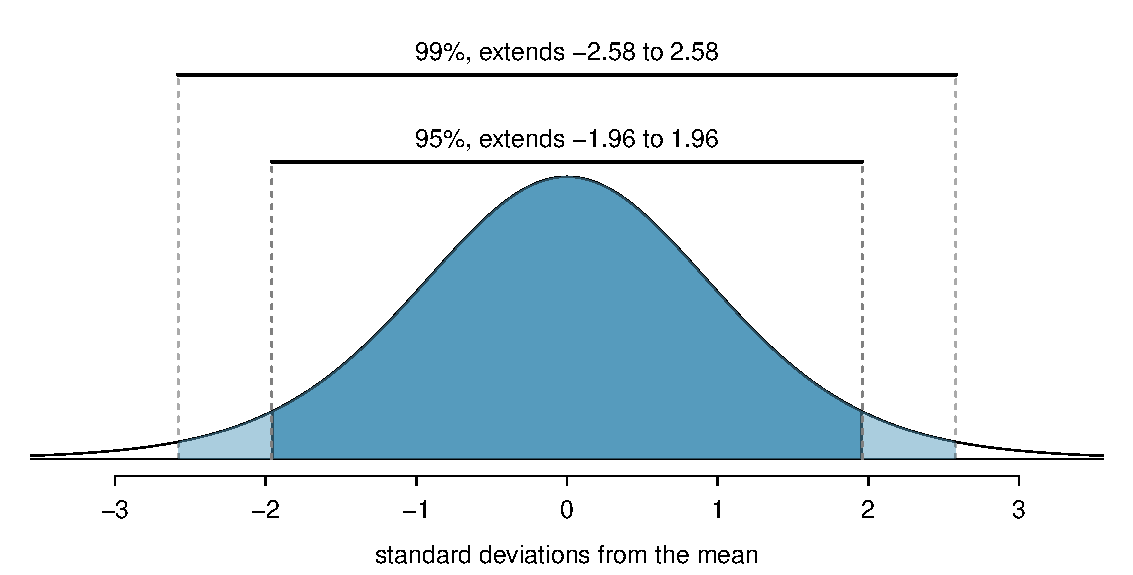
\includegraphics[width=\textwidth]
	{ch_inference_foundations_oi_biostat/figures/choosingZForCI/choosingZForCI}
	\caption{The area between -$z^{\star}$ and $z^{\star}$ increases as $|z^{\star}|$ becomes larger. If the confidence level is 99\%, $z^{\star}$ is chosen such that 99\% of the normal curve is between -$z^{\star}$ and $z^{\star}$, which corresponds to 0.5\% in the lower tail and 0.5\% in the upper tail: $z^{\star}=2.58$.}
	\label{choosingZForCI}
	\index{confidence interval!confidence level|)}
\end{figure}
 
A 99\% confidence interval will have the form 
\begin{align}
	\overline{x} \pm \ 2.58 \times \text{SE},
\end{align}
 and will consequently be wider than a 95\% interval for $\mu$ calculated from the same data, since the margin of error $m$ is larger.

% WARNING !!!!
% EOCE 4.9 (as of 2nd Edition) references the results of this exercise
\begin{example} {
	Create a 99\% confidence interval for the average days active per week of all YRBSS students using \data{yrbss.samp}. The point estimate is $\overline{x}_{active} = 3.75$ and the standard error is $SE_{\overline{x}} = 0.26$.}
Apply the 99\% confidence interval formula: $\overline{x}_{active}\ \pm\ 2.58 \times  SE_{\overline{x}} \rightarrow (3.08, 4.42)$. We are 99\% confident that the average days active per week of all YRBSS students is between 3.08 and 4.42~days.
\end{example}
%library(openintro); data(yrbss.samp); d <- yrbss.samp; mean(d$age); sd(d$age)/sqrt(100)

Previously, the 95\% confidence interval for the average days active per week of the students in YRBSS was calculated as (3.24, 4.26) days. Increasing the confidence level to 99\% results in (3.08, 4.42) days, which is a wider interval that is more likely to contain the population mean $\mu$. However, increasing confidence level comes at a cost: a wide interval is less informative in regards to providing a precise estimate of the population mean. Consider the extreme: to be "100\% confident" that an interval contains $\mu$, the interval must span all possible values of $\mu$. For example, it can be said with 100\% confidence that the average days active per week is between 0 and 7 days; while this interval necessarily contains $\mu$, it has no interpretive value and is completely uninformative. 

Decreasing confidence level results in a more precise estimate, but the interval has less chance of containing $\mu$. For example, consider a 50\% confidence interval for average days active per week using \data{yrbss.samp}: the $z^{\star}$ value is 0.67, and the confidence interval is (3.57, 3.92). This interval provides the most precise estimate of $\mu$, but there is only a 50\% chance that it contains $\mu$.

The choice of confidence level is a trade-off between obtaining a precise estimate and calculating an interval that contains the population parameter. In published literature, the most used confidence intervals are the 90\%, 95\%, and 99\%. 

\subsection{One-sided confidence intervals}
\label{onesidedCIs}

One-sided confidence intervals for a population mean provide either a lower bound or an upper bound, but not both.  One-sided confidence intervals have the form
\[
(\overline{x} - m, \infty) \text{ or } (-\infty, \overline{x} + m).
\]

While the margin of error $m$ for a one-sided interval is still calculated from the standard error of $\overline{x}$ and a $z^\star$ value, the choice of $z^\star$ is a different than for a two-sided interval. For example, the intent of a 95\% one-sided upper confidence interval is to provide an upper bound $m$ such that a data analyst can be 95\% confident that a population mean $\mu$ is less than $\overline{x} + m$. The $z^\star$ value must correspond with the point on the normal distribution that has 0.05 area in the right tail, $z^{\star} = 1.645$.\footnote{Previously, with a two-sided interval, 1.96 was chosen in order to have a total area of 0.05 from both the right and left tails.} A one-sided upper 95\%  confidence interval will have the form
\begin{align*}
(-\infty, \overline{x} + 1.645 \times \text{SE}).
\end{align*}

\begin{example}
	{Calculate a lower 95\% confidence interval for the average number of days active per week for high-school aged youth in the United States. In a sample of 100 students, the mean and standard error are $\overline{x} = 3.75$ and $SE = 0.26$ days.}
	
The lower 95\% bound is $3.75 - (1.645 \times 0.26) = 3.32$. Based on these data, we can be 95\% confident that the population days active per week among high-school aged youth in the US is at least 3.32 days.
\end{example}

%JV: Needs explanation about when to use one-sided interval versus two-sided.

\subsection{Interpreting confidence intervals}
\label{interpretingCIs}

\index{confidence interval!interpretation|(}

The correct interpretation of a confidence interval is, "We are XX\% confident that the population parameter is between \dots" While it may be tempting to say that a confidence interval captures the population parameter with a certain probability, this is a common error. The confidence level only quantifies how plausible it is that the parameter is within the interval; there is no probability associated with whether a parameter is contained in a specific confidence interval. The confidence coefficient reflects the nature of a procedure that is correct XX\% of the time, given that the assumptions in making the calculations are true.

The conditions about the validity of the normal approximation can be checked using the numerical and graphical summaries discussed in Chapter 1. However, the condition that data should be from a random sample is sometimes overlooked. If the data are not from a random sample, then the confidence interval no longer has interpretive value, since there is no population mean to which the confidence interval applies. For example, while only simple arithmetic is needed to calculate a confidence interval for BMI from the \data{famuss} dataset in Chapter 1, the participants in the study are almost certainly not a random sample from some population.

\begin{example}{Do Americans tend to be overweight? Body mass index (BMI) is one measure of body weight that adjusts for height. The National Health and Nutrition Examination Survey (NHANES) consists of a set of surveys and measurements conducted by the US CDC to assess the health and nutritional status of adults and children in the United States. The dataset \data{nhanes.samp} contains 76 variables and is a random sample of 200 individuals from the measurements collected in the years 2009-2010 and 2012-2013.\footnote{The sample was drawn from a larger sample of 20,293 participants in the \textbf{NHANES} package, available from The Comprehensive R Archive Network (CRAN). The CDC uses a complex sampling design that samples some demographic subgroups with larger probabilities, but \data{nhanes.samp} has been adjusted so that it can be viewed as a random sample of the US population.} Use \data{nhanes.samp} to calculate a 95\% confidence interval for adult BMI in the US population. \label{exNhanesBmi}}
	
	\begin{figure}[h]
		\centering
		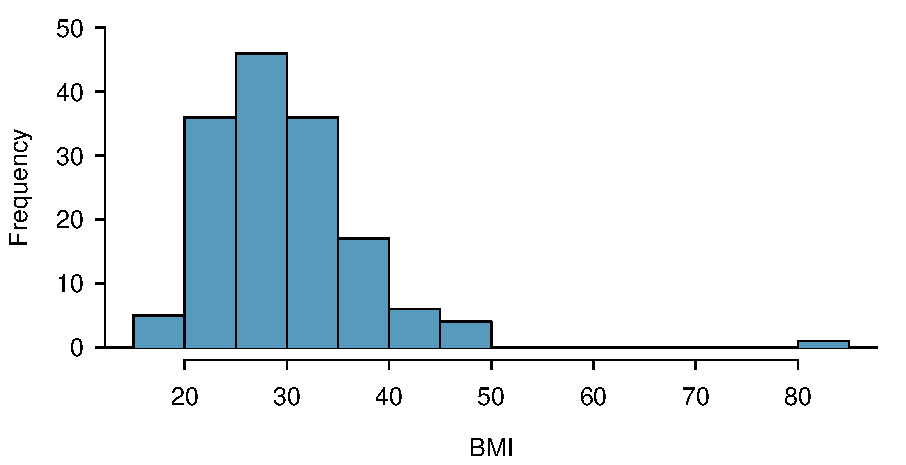
\includegraphics[width=\textwidth]
		{ch_inference_foundations_oi_biostat/figures/nhanesAdultBmiHist/nhanesAdultBmiHist}
		\caption{The distribution of the variable \var{BMI} for adult participants in NHANES.}
		\label{nhanesAdultBmiHist}
	\end{figure}
	
	In the random sample of 200 participants, BMI is available for 151 of the 152 participants that are 21 years of age or older. As shown in the histogram (Figure~\ref{nhanesAdultBmiHist}), the data are right-skewed, with one large outlier. The outlier corresponds to an implausibly extreme BMI value of 81.3; since it seems likely that the value represents an error when the data was recorded, this data point is excluded from the following analysis. 
	
	The mean and standard deviation in this sample of 150 are 29.7 and 7.7 $\text{kg}/\text{meter}{^2}$, respectively.  The sample size is large enough to justify using the normal approximation when computing the confidence interval.  The standard error of the mean is $\text{SE} = 7.7/\sqrt{150} = 0.63$, so the 95\% confidence interval is given by 
	\begin{align*}
	\overline{x}_{\text{BMI}} \pm (1.96)(\text{SE}) &= 29.7 \pm (1.96)(0.63) \\
	&= (28.5, 30.9).
	\end{align*}	
	
	Based on this sample, a data analyst can be 95\% confident that the average BMI of US adults is between 28.5 and 30.9 $\text{kg}/\text{m}{^2}$.
\end{example}

The World Health Organization (WHO) and other agencies use BMI to set normative guidelines for body weight. The current guidelines are shown in Table~\ref{whoBmiGuidelines}. 

%\footnote{\url{http://apps.who.int/bmi/index.jsp?introPage=intro_3.html}}. 

\begin{table}[h!]
	\begin{center}
		\begin{tabular}{|c|c|}
			\hline 
			Category & BMI range\tabularnewline
			\hline 
			\hline 
			Underweight & $<18.50$\tabularnewline
			\hline 
			Normal (healthy weight) & 18.5-24.99\tabularnewline
			\hline 
			Overweight & $\geq 25$\tabularnewline
			\hline 
			Obese & $\geq30$\tabularnewline
			\hline
		\end{tabular}
		\caption{WHO body weight categories based on BMI.} 
		\label{whoBmiGuidelines}
	\end{center}
\end{table}

The confidence interval (28.5, 30.9) $\text{kg}/\text{m}{^2}$ certainly suggests that the average BMI in the US population is higher than 21.7, the middle of the range for normal BMIs, and even higher than 24.99, the upper limit of the normal weight category. However, it is possible that the population average is outside the interval estimate, even though that would be inconsistent with the data in this particular sample. By random chance, a sample may have been selected in which individuals with high BMI are overrepresented, causing the sample mean to be higher than the population mean. What is the likelihood of observing a sample mean as large as 29.7 if the population average BMI in the US is actually 21.7? To address this question, it is necessary to use a tool of inference other than the confidence interval: hypothesis testing.

\index{confidence interval!interpretation|)}
\index{confidence interval|)}

\begin{comment}

%JV: older version of one-sided CI section

\subsection{One-sided confidence intervals}
\label{onesidedCIs}

One-sided confidence intervals for a population mean provide just a lower bound or an upper bound, but not both.  One-sided lower confidence intervals have the form
\[
    \overline{x} - m;
\]
one-sided upper confidence intervals are of the form 
\[
    \overline{x} + m.
\]
One-sided intervals less often used that two-sided intervals by they can be useful in some settings.

The margin of error $m$ for a one-sided interval is calculated slightly differently than a two-sided interval.  The intent of a 95\% one-sided upper confidence interval, for instance, is to provide an upper bound $m$ so that a data analyst can be 95\% confident that a population mean $\mu$ is less than $\overline{x} + m$.  Since all of the possible 5\% error lies to the right of $\overline{x} + m$, the calculation of $m$ uses the point on the normal distribution that has 0.05 area in the right tail, $z^{*} = 1.645$ instead of 1.96 in the two-sided interval.  A one-sided upper 95\%  confidence interval will have the form
\begin{align*}
	\overline{x} + z^{*} \frac{s}{\sqrt{n}} = \overline{x} + 1.645 \frac{s}{\sqrt{n}}.
\end{align*}
The upper bound in a one-sided interval will be closer to $\overline{x}$ than the upper bound in a two-sided interval with the same confidence coefficient, but there  will be no lower bound.  

A lower one-sided interval for a mean $\mu$ will be of the form
\begin{align*}
  \overline{x} - z^{*} \frac{s}{\sqrt{n}}.
\end{align*}

\begin{example}

Using the NHANES BMI data, calculate a lower 95\% confidence bound for average BMI.  A one-sided lower bound is found by calculating the lower confidence interval. For the 150 observations in the BMI data, the mean and standard deviation are $\overline{x} = 29.7$  $s = 7.7$ kg/meter$^2$.  The lower 95\% bound is $29.9 - 7.7/\sqrt{150} = 29.27$. Based on these data, we can be 95\% confident that the population mean BMI among US adults is at least 29.27 kg/meter$^{2}$.\end{example}

\textit{a bit more here about when to use what, or perhaps defer that to later}

\end{comment}

\section[Hypothesis testing]{Hypothesis testing} %\sectionvideohref{youtube-NVbPE1_Cbx8&list=PLkIselvEzpM7Pjo94m1e7J5jkIZkbQAl4}}
\label{hypothesisTesting}

\index{hypothesis testing|(}

Hypothesis testing is a method for calculating the probability of making a specific observation under a working hypothesis, called the null hypothesis. When testing a statistical hypothesis, one assumes that the data come from a distribution specified by the null hypothesis in order to calculate the likelihood of observing a value as extreme as the one represented by the sample. If the chances of such an extreme observation are small, there is enough evidence to reject the null hypothesis in favor of an alternative hypothesis. 

\begin{termBox}{\tBoxTitle{Null and alternative hypotheses}
		{The \term{null hypothesis ($H_0$)} often represents either a skeptical perspective or a claim to be tested. The \term{alternative hypothesis ($H_A$)} is an alternative claim and is often represented by a range of possible parameter values.}}
\end{termBox}

Generally, the investigator believes or suspects that the null hypothesis is not true and performs a hypothesis test in order to evaluate the strength of the evidence against the null hypothesis. The logic behind rejecting or failing to reject the null hypothesis is similar to the principle of presumption of innocence in many legal systems. In the United States, a defendant is assumed innocent until proven guilty; a verdict of guilty is only returned if it has been established beyond a reasonable doubt that the defendant is not innocent.


\begin{comment}

%JV: previous version of intro

Hypothesis testing is a method for calculating how unlikely an observation is under a working hypothesis, called the null hypothesis.  When testing a statistical hypothesis, one assumes that the data come from a distribution specified by the null hypothesis, calculates the likelihood that a statistic (called a test statistic) will have a value as extreme as the value observed if the data were drawn from the null hypothesis distribution, and rejects the null hypothesis only when that likelihood is small.  Hypothesis testing can be approached either informally or formally; while both methods reach essentially  the same conclusions, each has distinct advantages. The formal method provides a direct estimate of the strength of evidence against the working hypothesis, while the less formal approach can sometimes lead to a better understanding of the logic behind hypothesis testing.

The informal approach is based on what is known about a sample mean and its variability. Hypothesis testing starts with a null hypothesis, in this case, that the US population BMI matches the midpoint of the normal range, 21.7. Under this assumption, the mean of the hypothetical sampling distribution for the sample average of BMI will also be 21.7. The standard error of the sample mean is an approximate measure of how far the sample mean $\overline{x}_{\text{BMI}}$ is from the center of a distribution with population mean 21.7. In this example, $(\overline{x}_{\text{BMI}} - \mu_{\text{BMI}})/s =  (29.7 - 21.7)/0.63 = 12.7$.  The observed sample mean is 12.7 standard deviations to the right of 21.7. The sampling distribution of $\overline{x}_{\text{BMI}}$ is well approximated by a normal distribution. For a normally distributed random variable, the area to the right of 12.7 standard deviation units from the mean is less than 0.001; the likelihood of a sample with such an extreme mean, if the population is actually centered at 21.7, is vanishingly small. The event is so unusual that it is reasonable to conclude that the working hypothesis is wrong -- the data suggest that population average BMI is larger than 21.7.

The formal approach also starts with null hypothesis and adds an alternative claim that will be true if the null hypothesis is wrong. In nearly all scientific investigations, the investigator believes or suspects that the null hypothesis is not true and conducts a study to establish evidence for his or her conjecture.

\begin{termBox}{\tBoxTitle{Null and alternative hypotheses}
{The \term{null hypothesis ($H_0$)} often represents either a skeptical perspective or a claim to be tested. The \term{alternative hypothesis ($H_A$)} is an alternative claim and is often represented by a range of possible parameter values.}}
\end{termBox}

In the formal approach, the null hypothesis ($H_0$) is not rejected unless the evidence contradicting it is so strong that the only reasonable conclusion is to reject $H_0$ in favor of $H_A$. The logic is similar to the principle of presumption of innocence in many legal systems. In the United States, a defendant is assumed innocent until proven guilty; a verdict of guilty is only returned if it has been established beyond a reasonable doubt that the defendant is not innocent (i.e., guilty). 

The next section presents the steps of formal hypothesis testing.

\end{comment}

\subsection{The Formal Approach to Hypothesis Testing}
\label{formalHypothesisTesting}

In this section, hypothesis testing will be used to address the question of interest: Do Americans tend to be overweight? More precisely, what is the likelihood of observing a sample mean as large as 29.7 (as calculated from \data{nhanes.samp}) if the population average BMI in the US is actually 21.7?

\subsubsection{Step 1: Formulating null and alternative hypotheses}

The claim to be tested is that the population average BMI in the US is 21.7. Thus, the null hypothesis can be written as:

\[H_0: \mu_{\text{bmi}} = 21.7\]

Due to the extensive literature documenting high obesity rates in the United States, it is reasonable to assume that if $H_0$ is not true, the population average BMI would be larger than 21.7: 

\[H_A: \mu_{\text{bmi}} > 21.7\]

The alternative hypothesis $H_A: \mu_{\text{bmi}} > 21.7$ is called a \term{one-sided alternative}.\footnote{The null hypothesis in this setting is sometimes written as $H_0: \mu_{\text{bmi}} \leq 21.7$, since the alternative hypothesis is one-sided, but that notation will not be used in this text.} An investigator studying a similar problem in a different setting, such as for a region where drought has led to food shortages, might formulate the alternative as $ H_A:\mu_{\text{bmi}} < 21.7$ under the assumption that population BMI is likely lower than normal. In other settings where income inequality causes substantial disparities in access to food between subgroups of the population, it might be more appropriate to use a \term{two-sided alternative}, $\mu_{\text{bmi}} \neq 21.7$. 

More generally, when testing a hypothesis about a population mean $\mu$, the null and alternative hypotheses for a one-sided alternative are written as follows

\begin{itemize}
	\item For a one-sided alternative: \[H_0: \mu = \mu_0, \ H_A: \mu < \mu_0\] or \[H_0: \mu = \mu_0, \  H_A: \mu > \mu_0;\]
	
	\item For a two-sided alternative: \[H_0: \mu = \mu_0, \ H_A: \mu \neq \mu_0.\]
\end{itemize}

The symbol $\mu$ denotes a population mean, while $\mu_0$ refers to the numeric value specified by the null hypothesis; $\mu_0 = 21.7$ in this example. Note that null and alternative hypotheses are statements about the underlying population, not the observed values from a sample. 

\subsubsection{Step 2: Specifying a significance level, $\alpha$}

It is important to specify how rare or unlikely an event must be in order to represent sufficient evidence against the null hypothesis. This should be done during the design phase of a study, to prevent any bias that could result from only defining 'rare' after analyzing the results. 

When testing a statistical hypothesis, an investigator specifies a \term{significance level}, $\alpha$, that defines a 'rare' event. Typically, $\alpha = 0.05$, though it may be larger or smaller, depending on context; this is discussed in more detail in Section~\ref{significanceLevel}. An $\alpha$ level of $0.05$ means that an event occurring with probability lower than 5\% will be considered sufficient evidence against $H_0$.

\begin{comment}

%JV: previous draft

For the \data{nhanes.samp} BMI data, the observed sample mean was more than 12 standard deviations to the right of the population mean specified in $H_0$ -- an undeniably extreme observation. In contrast, if the sample mean had only been 2 standard deviations to the right of 21.7, it would have been less obvious whether observing a sample mean 2 or more standard deviations larger than 21.7 qualified as a rare enough event to reject the null hypothesis. 

When testing a statistical hypothesis, an investigator specifies a \term{significance level}, $\alpha$, that defines "rare". Typically, $\alpha = 0.05$, though it may be larger or smaller, depending on context; this is discussed in more detail in Section~\ref{significanceLevel}. The value of $\alpha$ will be compared with the probability that the sample mean is as or more extreme under the null hypothesis.

It is important to specify in the design of a study how rare an event must be in order to represent sufficient evidence against $H_0$.  Otherwise, it is tempting to define `rare' using the likelihood of the observed data, because many outcomes could be deemed rare `post hoc' by redefining the notion of rare.  This is akin to adding lines to a tennis court after one player has hit a questionable serve -- any serve can be made `good' by adjusting the lines to the serve. 

\end{comment}

\subsubsection{Step 3: Calculating the test statistic}

Calculating the test statistic $t$ is analogous to standardizing observations with Z-scores as discussed in Chapter 3. The test statistic quantifies the number of standard deviations between the sample mean $\overline{x}$ and the population mean $\mu$:

\begin{align*}
t=\frac{\overline{x}-\mu_0}{s/\sqrt{n}},
\end{align*}

where $s$ is the sample standard deviation and $n$ is the number of observations in the sample. For the 150 adult responses in \data{nhanes.samp}, $\overline{x} = 29.7$, $s = 7.7$, so the test statistic is calculated as follows:

\[t = \frac{29.7 - 21.7}{7.7/\sqrt{150}} = 12.7.\]
The observed sample mean is 12.7 standard deviations to the right of the $\mu_0 = 21.7$.

\subsubsection{Step 4: Calculating the $p$-value}

The \term{$p$-value} is the probability of observing a sample mean as or more extreme than the observed value, under the assumption that the null hypothesis is true. In samples of size 40 or more, the $t$-statistic will have a standard normal distribution unless the data are strongly skewed or extreme outliers are present. Recall that a standard normal distribution has mean 0 and standard deviation 1.

For one-sided tests with $H_A: \mu > \mu_0$, the $p$-value is given by $P(Z \geq t)$, as shown in Figure~\ref{pValueOneSided}. If $H_A: \mu < \mu_0$, the $p$-value is the area to the left of the $t$-statistic, $P(Z \leq t)$.

\begin{figure}[h]
	\centering
	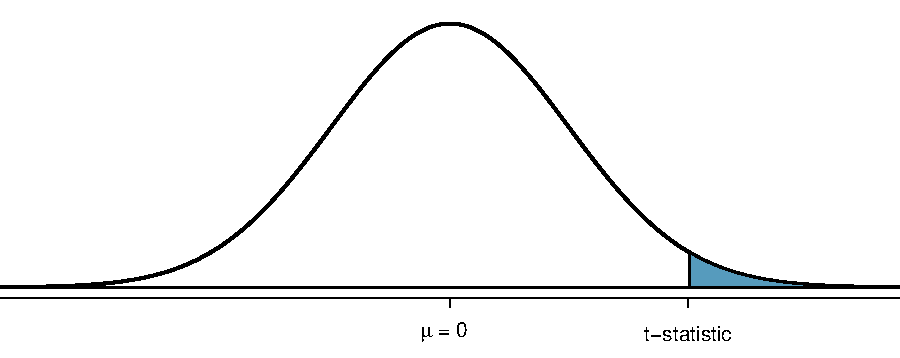
\includegraphics[width=0.9\textwidth]{ch_inference_foundations_oi_biostat/figures/pValueOneSided/pValueOneSided}
	\caption{A one-sided $p$-value for $H_A: \mu > \mu_0$ is represented on a standard normal distribution as the shaded area to the right of the $t$-statistic. This area equals the probability of an observation as or more extreme than $\overline{x}$.}
	\label{pValueOneSided}
\end{figure}

For two-sided tests, with $H_A: \mu \neq \mu_0$, the $p$-value is the sum of the area of the two tails defined by the $t$-statistic: $P(Z \leq -t) + P(Z \geq t) = P(Z \geq |t| )$ (Figure~\ref{pValueTwoSided}).

\begin{figure}[h]
	\centering
	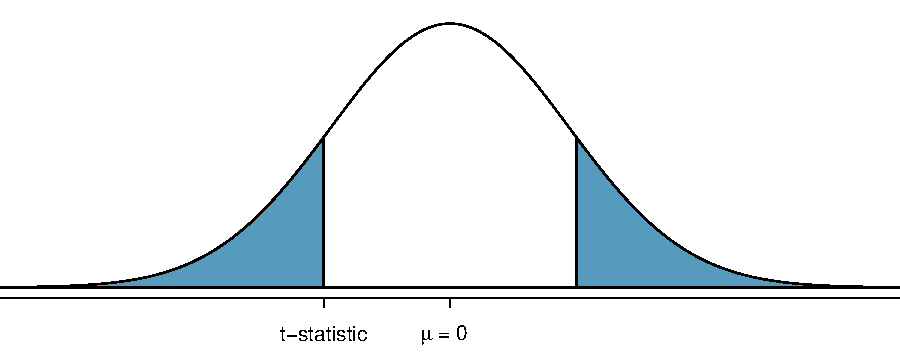
\includegraphics[width=0.9\textwidth]{ch_inference_foundations_oi_biostat/figures/pValueTwoSided/pValueTwoSided}
	\caption{A two-sided $p$-value for $H_A: \mu \neq \mu_0$ on a standard normal distribution. The shaded regions represent observations as or more extreme than $\overline{x}$ in either direction.}
	\label{pValueTwoSided}
\end{figure}

The $p$-value can either be calculated from software or from the normal probability tables. For the BMI example, the $p$-value is vanishingly small: $p = P(Z \geq 12.7) < 0.001$.

\subsubsection{Step 5: Drawing a conclusion}

To reach a conclusion about the null hypothesis, directly compare $p$ and $\alpha$. Note that for a conclusion to be informative, it must be presented in the context of the original question; it is not useful to simply state whether $H_0$ is rejected or not.

If $p > \alpha$, the observed sample mean is not extreme enough to warrant rejecting $H_0$; more formally stated, there is insufficient evidence to reject $H_0$. A high $p$-value suggests that the difference between the observed sample mean and $\mu_0$ can reasonably be attributed to random chance.

If $p \leq \alpha$, there is sufficient evidence to reject $H_0$ and accept $H_A$. In the \data{nhanes.samp} BMI data, the $p$-value is extremely small, with the $t$-statistic lying far to the right of the population mean. The chance of drawing a sample with mean of 29.7 if the distribution were actually centered at 21.7 is less than 0.001! Thus, the data support the conclusion that the average BMI in the United States is larger than 21.7. 

\begin{exercise}
Suppose that the mean BMI in the sampled group of 150 adults was actually 22.5. Would there still be enough evidence at the $\alpha = 0.05$ level to reject $H_0: \mu_{\text{bmi}} = 21.7$ in favor of $H_A: \mu_{\text{bmi}} > 21.7$?\footnote{Re-calculate the $t$-statistic: $(22.5 - 21.7)/(7.7/\sqrt{150}) = 1.27$. The $p$-value $P(Z \geq 1.27) = 0.102$. Since $p$ > $\alpha$, there is insufficient evidence to reject $H_0$. The observed difference between $\overline{x}$ and 21.7 is likely due to chance.}
\end{exercise}

\subsection{Two examples}


\begin{example}
{While fish and other types of seafood are important to a healthy diet, nearly all fish and shellfish contain traces of mercury. Dietary exposure to mercury can be particularly dangerous for young children and unborn babies. Regulatory organizations such as the US Food and Drug Administration (FDA) provide guidelines as to which types of fish have particularly high levels of mercury and should be completely avoided by pregnant women and young children; additionally, certain species known to have low mercury levels are recommended for consumption. While there is no international standard that define excessive mercury levels in saltwater fish species, general consensus is that fish with levels above 0.5 parts per million (ppm) should not be consumed. A study conducted to assess mercury levels for saltwater fish caught off the coast of New Jersey found that a sample of 23 bluefin tuna had mean mercury level of 0.52 ppm, with standard deviation 0.16 ppm.\footnote{J. Burger, M. Gochfeld, Science of the Total Environment 409 (2011) 1418–1429} Suppose that the FDA has asked you to analyze this data -- should bluefin tuna from New Jersey be added to the list of species recommended for consumption, or should a warning be issued about their mercury levels?}
\label{hypTestTuna}

Let $\mu$ be the population average mercury content for bluefin tuna caught off the coast of New Jersey. Conduct a two-sided test of the hypothesis $\mu = 0.50$ ppm in order to assess the evidence for either definitive safety or potential danger.

\textit{Formulate the null and alternative hypotheses}. $H_0: \mu = 0.50$ ppm vs. $H_A: \mu \neq 0.50$ ppm

\textit{Specify the significance level, $\alpha$}.  A significance level of $\alpha = 0.05$ seems reasonable. 

\textit{Calculate the test statistic}. The  $t$-statistic has value
\begin{align*}
t &= \frac{\overline{x}-\mu_0}{s/\sqrt{n}} = \frac{0.53 - 0.50} {0.16/\sqrt{23}} = 0.859.
\end{align*}

\textit{Calculate the $p$-value}.

For this two-sided alternative $H_A: \mu \neq 0.50$, the $p$-value will be 

\[P(Z \leq -t) + P(Z \geq t)= 2P(Z \leq - 0.859) = 0.390.\]

\begin{figure}[h]
	\centering
	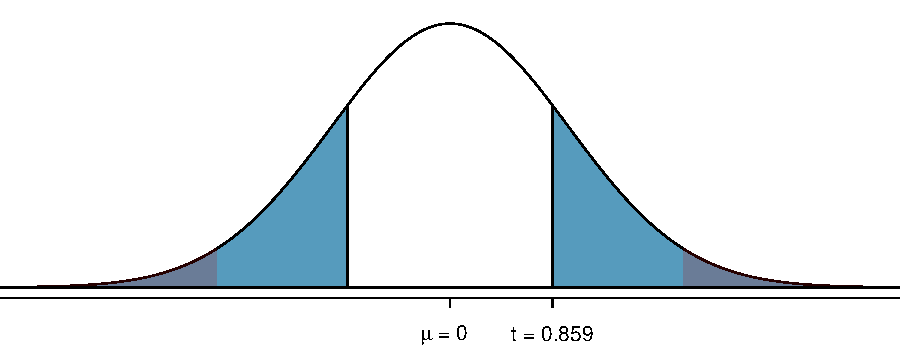
\includegraphics[width=0.9\textwidth]{ch_inference_foundations_oi_biostat/figures/pValueTuna/pValueTuna}
	\caption{The blue shaded region represents the $p$-value, the area to the right of $t = 0.859$ and to the left of $-t = -0.859$. The grey shaded region represents the \term{rejection region} as defined by $\alpha$; in this case, an area of 0.025 in each tail. The $t$-statistic calculated from $\overline{x}$ would have to lie within either of the grey regions in order to constitute sufficient evidence against the null hypothesis.}
	\label{pValueTuna}
\end{figure}

\textit{Draw a conclusion}. The $p$-value is larger than the specified significance level $\alpha$, as shown in Figure~\ref{pValueTuna}.\footnote{The grey shaded regions are bounded by -1.96 and 1.96, since the area within 1.96 standard deviations of the mean captures 95\% of the distribution.} The null hypothesis is not rejected since the data do not show that the mercury content of bluefin tuna caught off the coast of New Jersey differs significantly from 0.5 ppm. From these data, there is not statistically significant evidence to either recommend these fish as clearly safe for consumption or to warn consumers against eating them. Based on these data, the Food and Drug Administration might decide to monitor this species more closely and conduct further studies. 

From the available evidence, we failed to reject the null hypothesis that the mean mercury level for the New Jersey coastal population of bluefin tuna is 0.5 ppm. However, "failure to reject" is not equivalent to "accepting" the null hypothesis. Recall the earlier analogy related to the principle of "innocent until proven guilty". If there is not enough evidence to prove that the defendant is guilty, the official decision must be "not guilty", since the defendant may not necessarily be innocent. Similarly, while there was not enough evidence to suggest that $\mu$ is not equal to 0.5 ppm, it would be incorrect to claim that the evidence states that $\mu$ \textit{is} 0.5 ppm.

\end{example}

\newpage

\begin{example}
{In 2015, the National Sleep Foundation published new guidelines for the amount of sleep recommended for adults: 7-9 hours of sleep per night.\footnote{Sleep Health: Journal of the National Sleep Foundation, Vol. 1, Issue 1, p40 - 43} The NHANES survey includes a question asking respondents about how many hours per night they sleep; the responses are available in \data{nhanes.samp}, the data used earlier to investigate BMI. In the sample of 151 adults, the average reported hours of sleep is 7.18, with standard deviation 1.33. Is there evidence that American adults sleep less than 7 hours per night?}

Let $\mu$ be the population average of hours of sleep per night for US adults. Conduct a one-sided test, since the question asks whether the average amount of sleep per night might be less than 7 hours. 

\textit{Formulate the null and alternative hypotheses}. $H_0: \mu = 7$ hours vs. $H_A: \mu < 7$ hours

\textit{Specify the significance level, $\alpha$}.  Let $\alpha = 0.05$, since the question does not reference a different value. 

\textit{Calculate the test statistic}. The $t$-statistic has value
\[t = \frac{\overline{x}-\mu_0}{s/\sqrt{n}} = \frac{7.18 - 7.00} {1.33/\sqrt{151}} = 1.65.\]

\textit{Calculate the $p$-value}.

For this one-sided alternative $H_A: \mu < 7$, the $p$-value will be 

\[P(Z \leq t) = P(Z < 1.65) = 0.95.\]

Note that this $p$-value is relatively large, and much greater than 0.05. Instead of observing a value of $\overline{x}$ that is smaller than $\mu_0 = 7$, the value is larger than 7. 

A common error when conducting one-sided tests is to assume that the $p$-value will always be the area in the smaller of the two tails to the right or left of the observed value. It is important to remember that the area must correspond to the direction specified by the alternative hypothesis. Since the alternative states that $\mu_0$ is less than 7, the $p$-value is represented by the area to the left of $t = 1.65$, as shown in Figure~\ref{pValueSleep}.

\begin{figure}[h]
	\centering
	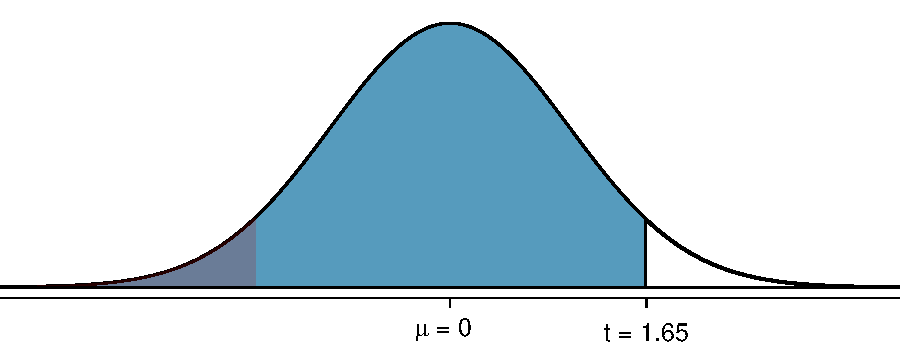
\includegraphics[width=0.9\textwidth]{ch_inference_foundations_oi_biostat/figures/pValueSleep/pValueSleep}
	\caption{The blue shaded region represents the $p$-value, the area to the left of $t = 1.65$. The grey shaded region represents the rejection region of area 0.05 in the left tail.}
	\label{pValueSleep}
\end{figure}

\textit{Draw a conclusion}.  The $p$-value is larger than the specified significance level $\alpha$. The null hypothesis is not rejected since the data do not contain evidence to support the claim that American adults sleep less than 7 hours per night.

\end{example}

\begin{exercise}
	From these data, is there sufficient evidence at the $\alpha = 0.10$ significance level to support the claim that American adults sleep more than 7 hours per night?\footnote{The $t$-statistic does not change from 1.65. Re-calculate the $p$-value since the alternative hypothesis is now $H_A: \mu > 7$: $P(Z \geq 1.65) = 0.05$. Since $p$ < $\alpha$, there is sufficient evidence to reject $H_0$ at $\alpha = 0.10$ and accept the alternative hypothesis that American adults sleep more than 7 hours per night. This can be visualized below; the $t$-statistic falls within the rejection region (shaded red).\\
	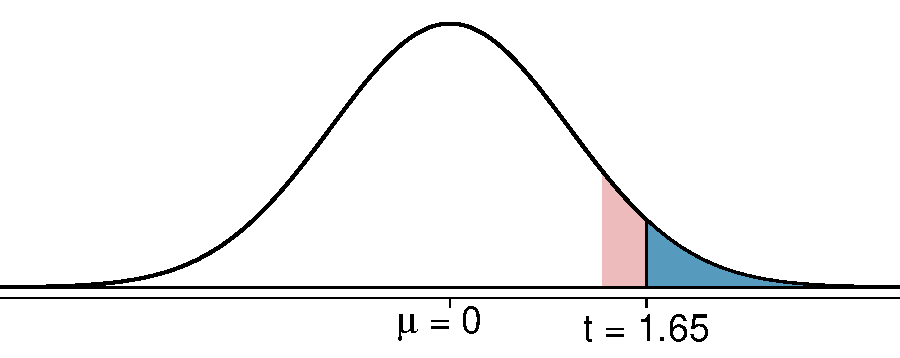
\includegraphics[width=0.3\textwidth]{ch_inference_foundations_oi_biostat/figures/pValueSleep/pValueSleepEx}}
\end{exercise}

\subsection{Hypothesis testing and confidence intervals}

In a confidence interval for $\mu$, a potential population mean $\mu_0$ that falls outside the interval is inconsistent with the observed sample, since the interval is constructed based on information about $\overline{x}$ and $s$. In other words, it is unlikely that the sample would have been observed if the population distribution were actually centered at $\mu_0$. Hypothesis testing follows the same logic: a null hypothesis about $\mu_0$ is rejected if the observed sample mean is unlikely under $H_0$. This leads to a useful way to conduct significance tests based on confidence intervals.

The relationship between a hypothesis test and the corresponding confidence interval is defined by $\alpha$. Suppose that a two-sided test is conducted at significance level $\alpha$; the confidence level of the matching interval is (1 - $\alpha$)\%. For example, a two-sided hypothesis test with $\alpha = 0.05$ can be compared to a 95\% confidence interval. A hypothesis test will reject at $\alpha = 0.05$ if the 95\% confidence interval does not contain the null hypothesis value of the population mean ($\mu_0$).

\begin{termBox}{\tBoxTitle{The relationship between two-sided hypothesis tests and confidence intervals}
{When testing the null hypothesis $H_0:\mu = \mu_0$ against the two-sided alternative $H_A: \mu \neq \mu_0$, $H_0$ will be rejected at significance level $\alpha$ when the $100(1-\alpha)\%$ confidence interval for $\mu$ does not contain $\mu_0$. }}
\end{termBox}

\begin{example}
{Calculate the confidence interval for the average mercury level for bluefin tuna caught off the coast of New Jersey. The summary statistics for the sample of 21 fish are $\overline{x} = 0.53$ ppm and $s = 0.16$ ppm. Does the interval agree with the results of Example~\ref{hypTestTuna}?}

The 95\% confidence interval is: 

\[\overline{x} \pm 1.96 \dfrac{s}{\sqrt{n}}= 0.53 \pm 1.96 \frac{0.16}{\sqrt{21}} = (0.462, 0.598) \text{ ppm}.\]

The confidence interval is relatively wide, containing values below 0.5 ppm that might be regarded as safe, in addition to values that might be regarded as potentially dangerous. This interval supports the conclusion reached from hypothesis testing; the sample data does not suggest that the mercury level differs significantly from 0.5 ppm in either direction. 

\end{example}
	
The same relationship applies for one-sided hypothesis tests. For example, a one-sided hypothesis test with $\alpha = 0.05$ and $H_A: \mu > \mu_0$ corresponds to a one-sided 95\% confidence interval that has a lower bound, but no upper bound (i.e., ($\overline{x} - m, \infty$)).
	
\begin{termBox}{\tBoxTitle{The relationship between one-sided hypothesis tests and confidence intervals}
  {
  	\begin{itemize}
	\item When testing the null hypothesis $H_0:\mu = \mu_0$ against the one-sided alternative $H_A: \mu > \mu_0$, $H_0$ will be rejected at significance level $\alpha$ when $\mu_0$ is smaller than the lower bound of the $100(1-\alpha)\%$ confidence interval for $\mu$. This is equivalent to $\mu_0$ having a value outside the lower one-sided confidence interval ($\overline{x} - m, \infty$).

	\item When testing the null hypothesis $H_0:\mu = \mu_0$ against the one-sided alternative $H_A: \mu < \mu_0$, $H_0$ will be rejected at significance level $\alpha$ whenever $\mu_0$ is larger than the upper bound of the $100(1-\alpha)\%$ confidence interval for $\mu$. This is equivalent to $\mu_0$ having a value outside the upper one-sided confidence interval ($-\infty, \overline{x} + m$).
	\end{itemize}
  }}
\end{termBox}
		
\begin{example}
{Previously, a hypothesis test was conducted at $\alpha = 0.05$ to test the null hypothesis $H_0: \mu = 21.7$ against the alternative $H_A: \mu > 21.7$, for the average BMI of US adults. Calculate the corresponding confidence interval and compare the information obtained from a confidence interval versus a hypothesis test. The summary statistics for the sample of 150 adults are $\overline{x} = 29.7$ and $s = 7.7$.}	

The lower one-sided 95\% confidence interval is:

\[(\overline{x} - 1.645 \dfrac{s}{\sqrt{n}}, \infty) = (29.7 - 1.645\dfrac{7.7}{\sqrt{150}}, \infty) = (28.7, \infty) \]

From these data, we can be 95\% confident that the average BMI among US adults is at least 28.7. Since $\mu_0 = 21.7$ is outside the one-sided interval, there is sufficient evidence to reject the null hypothesis $H_0: \mu = 21.7$ at $\alpha = 0.05$. 

The interval provides a range of plausible values for a parameter based on the observed sample; in this case, the data suggest that the population average BMI for US adults is at least 28.7, well above the WHO body weight standard for overweight classification ($\geq 25$). The $p$-value from a hypothesis test represents a measure of the strength of the evidence against the null hypothesis, indicating how unusual the observed sample would be under $H_0$; the hypothesis test indicated that it is very unlikely ($p < 0.001$) that the population average is 21.7. 

In practice, both a $p$-value and a confidence interval are computed when using a sample to make inferences about a population parameter.

\end{example}

\subsection{Decision errors}

Hypothesis tests can potentially result in incorrect decisions, such as rejecting the null hypothesis when the null is actually true. Table~\ref{fourHTScenarios} shows the four possible ways that the conclusion of a test can be right or wrong.

\begin{table}[ht]
	\centering
	\begin{tabular}{l l c c}
		& & \multicolumn{2}{c}{\textbf{Test conclusion}} \\
		\cline{3-4}
		\vspace{-3.7mm} \\
		& & Fail to reject $H_0$ &  Reject $H_0$ in favor of $H_A$ \\
		\cline{2-4}
		\vspace{-3.7mm} \\
		& $H_0$ True & Correct Decision &  Type~1 Error \\
		\raisebox{1.5ex}{\textbf{Reality}} & $H_A$ True & Type~2 Error & Correct Decision\\
		\cline{2-4}
	\end{tabular}
	\caption{Four different scenarios for hypothesis tests.}
	\label{fourHTScenarios}
\end{table}

Rejecting the null hypothesis when the null is true is referred to as a \term{Type I error}, while a \term{Type II error} refers to failing to reject the null hypothesis when the alternative is true. 

\begin{example}
{In a trial, the defendant is either innocent ($H_0$) or guilty ($H_A$). After hearing evidence from both the prosecution and the defense, the court must reach a verdict. What does a Type~I Error represent in this context? What does a Type~II Error represent?}	
If the court makes a Type~I error, this means the defendant is innocent, but wrongly convicted (rejecting $H_0$ when $H_0$ is true). A Type~II error means the court failed to convict a defendant that was guilty (failing to reject $H_0$ when $H_0$ is false).		
\label{whatAreTheErrorTypesInUSCourts}	
\end{example}

The probability of making a Type I error is the same as the significance level $\alpha$, since $\alpha$ determines the cutoff point for rejecting the null hypothesis. For example, if $\alpha$ is set to 0.05, then there is a 5\% chance of incorrectly rejecting $H_0$. 

The rate of Type I error can be reduced by lowering $\alpha$ (e.g., to 0.01 instead of 0.05); doing so requires an observation to be more extreme to qualify as sufficient evidence against the null hypothesis. However, this inevitably raises the rate of Type II errors, since the test will now have a higher chance of failing to reject the null hypothesis when the alternative is true.

\begin{example}
{In a courtroom setting, how might the rate of Type I errors be reduced? What effect would this have on the rate of Type II errors?}	
Lowering the rate of Type I error is equivalent to raising the standards for conviction such that fewer people are wrongly convicted. This increases Type II error, since higher standards for conviction leads to fewer convictions for people who are actually guilty.
\end{example}


\begin{exercise} \label{howToReduceType2ErrorsInUSCourts}
	In a courtroom setting, how might the rate of Type II errors be reduced? What effect would this have on the rate of Type I errors?\footnote{To lower the rate of Type II error, the court could lower the standards for conviction, or in other words, lower the bar for what constitutes sufficient evidence of guilt (increase $\alpha$, e.g. to 0.10 instead of 0.05). This will result in more guilty people being convicted, but also increase the rate of wrongful convictions, increasing the Type I error.}
\end{exercise}

\index{hypothesis testing!decision errors|)}

\subsubsection{Choosing a significance level}

\index{hypothesis testing!significance level|(}
\index{significance level|(}

Reducing the error probability of one type of error increases the chance of making the other type. As a result, the significance level is often adjusted based on the consequences of any decisions that might follow from the result of a significance test.

\label{significanceLevel}

By convention, most scientific studies use a significance level of $\alpha = 0.05$; small enough such that the chance of a type I error is relatively rare (occurring on average 5 out of 100 times), but also large enough to prevent the null hypothesis from almost never being rejected. If a Type I error is especially dangerous or costly, a smaller value of $\alpha$ is chosen (e.g., 0.01). Under this scenario, it is better to be cautious about rejecting the null hypothesis, so very strong evidence against $H_0$ is required in order to reject the null and accept the alternative. Conversely, if a Type II error is relatively dangerous, then a larger value of $\alpha$ is chosen (e.g., 0.10). Hypothesis tests with larger values of $\alpha$ will reject $H_0$ more often.

For example, in the early stages of assessing a drug therapy, it may be important to continue further testing even if there is not very strong initial evidence for a beneficial effect. If the scientists conducting the research know that any initial positive results will eventually be more rigorously tested in a larger study, they might choose to use $\alpha = 0.10$ to reduce the chances of making a type II error: prematurely ending research on what might turn out to be a promising drug.

A government agency responsible for approving drugs to be marketed to the general population, however, would likely be biased towards minimizing the chances of making a type I error -- approving a drug that turns out to be unsafe or ineffective. As a result, they might conduct tests at significance level 0.01 in order to reduce the chances of concluding that a drug works when it is in fact ineffective. The US FDA and the European Medical Agency (EMA) customarily require that two independent studies show the efficacy of a new drug or regimen using $\alpha = 0.05$, though other values are sometimes used.

\index{significance level|)}
\index{hypothesis testing!significance level|)}
\index{hypothesis testing|)}

\subsection{Choosing between one-sided and two-sided tests}

In some cases, the choice of a one-sided or two-sided test can influence whether the null hypothesis is rejected. For example, consider a sample for which the $t$-statistic is 1.80. If a two-sided test is conducted at $\alpha = 0.05$, the $p$-value is given by

\[P(Z \leq -t) + P(Z \geq t)= 2P(Z \geq 1.80) = 0.072.\]

There is insufficient evidence to reject $H_0$, since $p > \alpha$. However, what if a one-sided test is conducted at $\alpha = 0.05$, with $H_A: \mu > \mu_0$? In this case, the $p$-value is given by

\[P(Z \geq t)= P(Z \geq 1.80) = 0.036.\]

The conclusion of the test is different: since $p < \alpha$, there is sufficient evidence to reject $H_0$ in favor of the alternative hypothesis. Figure~\ref{twoSidedTestConservative} illustrates the different outcomes from the tests.

\begin{figure}[h]
	\centering
	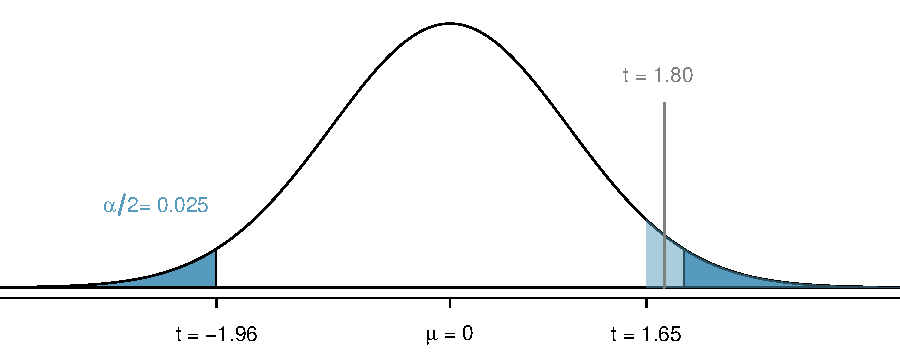
\includegraphics[width=0.9\textwidth]
	{ch_inference_foundations_oi_biostat/figures/twoSidedTestConservative/twoSidedTestConservative}
	\caption{Under a one-sided test at significance level $\alpha$ = 0.05, a $t$-statistic of 1.80 is within the rejection region (shaded light blue). However, it would not be within the rejection region under a two-sided test with $\alpha$ = 0.05 (darker blue).}
	\label{twoSidedTestConservative}
\end{figure}

Two-sided tests are more "conservative" than one-sided tests; it is more difficult to reject the null hypothesis with a two-sided test. The $p$-value for a one-sided test is exactly half the $p$-value for a two-sided test conducted at the same significance level; as a result, it is easier for the $p$-value from a one-sided test to be smaller than $\alpha$. Additionally, since the rejection region for a two-sided test is divided between two tails, a test statistic needs to be more extreme in order to fall within a rejection region. While the $t$-statistic of 1.80 is not within the two-sided rejection region, it is within the one-sided rejection region.\footnote{The two-sided rejection regions are bounded by -1.96 and 1.96, while the one-sided rejection region begins at 1.65.}

For a fixed sample size, a one-tailed test will have a smaller probability of type II error in comparison to a two-tailed test conducted at the same $\alpha$ level. In other words, with a one-sided test, it is easier to reject the null hypothesis if the alternative is actually true. 

The choice of test should be driven by context, although it is not always clear which test is appropriate. Since it is easier to reject $H_0$ with the one-tailed test, it might be tempting to always use a one-tailed test when a significant result in a particular direction would be interesting or desirable. 

However, it is important to consider the potential consequences of missing a significant difference in the untested direction. Generally, a two-sided test is the safest option, since it does not incorporate any existing biases about the direction of the results and can detect a difference at either the upper or lower tail. In the 1980s, researchers were interested in assessing a new set of drugs expected to be more effective at reducing heart arrhythmias than previously available therapies. They designed a one-sided clinical trial, convinced that the newer therapy would reduce mortality. The trial was quickly terminated due to an unanticipated effect of the drug; an independent review board found that the newer therapy was almost 4 times as likely to kill patients as a placebo! In a clinical research setting, it can be dangerous and even unethical to conduct a one-sided test in the belief that there is no possibility of patient harm from the drug intervention being tested.

%cite two_tailed_clinical

One-sided tests are appropriate if the consequences of missing an effect in the untested direction are negligible, or if a large observed difference in the untested direction and a conclusion of "no difference" lead to the same decision. For example, suppose that a company has developed a drug to reduce blood pressure that is cheaper to produce than current options available on the market. If the drug is shown to be equally effective or more effective than an existing drug, the company will continue investing in it. Thus, they are only interested in testing the alternative hypothesis that the new drug is less effective than the existing drug, in which case, they will stop the project. It is acceptable to conduct a one-sided test in this situation since missing an effect in the other direction causes no harm. 

The decision as to whether to use a one-sided or two-sided test must be made before data analysis begins, in order to avoid biasing conclusions based on the results of a hypothesis test. In particular, changing to a one-sided test after discovering that the results are "almost" significant for the two-sided test is unacceptable. Manipulating analyses in order to achieve low $p$-values leads to invalid results that are often not replicable. Unfortunately, this kind of "significance-chasing" has become widespread in published science, leading to concern that most current published research findings are false.

%cite statistical_errors
%cite published_research_false

\begin{comment}

%JV: I'm not convinced that this material on the CLT is strictly necessary for understanding inference, esp. since the use of the CLT is not emphasized in the earlier section.

\section[A closer look at the Central Limit Theorem]{A closer look at the Central Limit Theorem} %\sectionvideohref{youtube-lsCc_pS3O28&list=PLkIselvEzpM7Pjo94m1e7J5jkIZkbQAl4}}
\label{cltSection}

\index{Central Limit Theorem|(}

The normal probability model for the sample mean tends to be very good when the sample consists of at least 30 independent observations and the population data are not strongly skewed. The Central Limit Theorem provides the theory that supports this assumption.

\begin{termBox}{\tBoxTitle{Central Limit Theorem, informal definition}
The distribution of $\overline{x}$ is approximately normal. The approximation can be poor if the sample size is small, but it improves with larger sample sizes.}
\end{termBox}

%%% revisions to here, 7/5/16, 13:48

This section examines the accuracy of the normal model for the sample mean for three possible quantitative continuous population distributions:  a \emph{uniform} distribution, one an \emph{exponential} distribution, and a \emph{log-normal} distribution. These density functions for these distributions are shown in the top panels of Figure~\ref{cltSimulations}. The uniform distribution is symmetric, the exponential distribution has moderate skew -- its right tail is relatively short (few outliers), and the log-normal distribution is strongly skewed and will tend to produce more apparent outliers.\index{skew!example: moderate}\index{skew!example: strong}

\begin{figure}
   \centering
   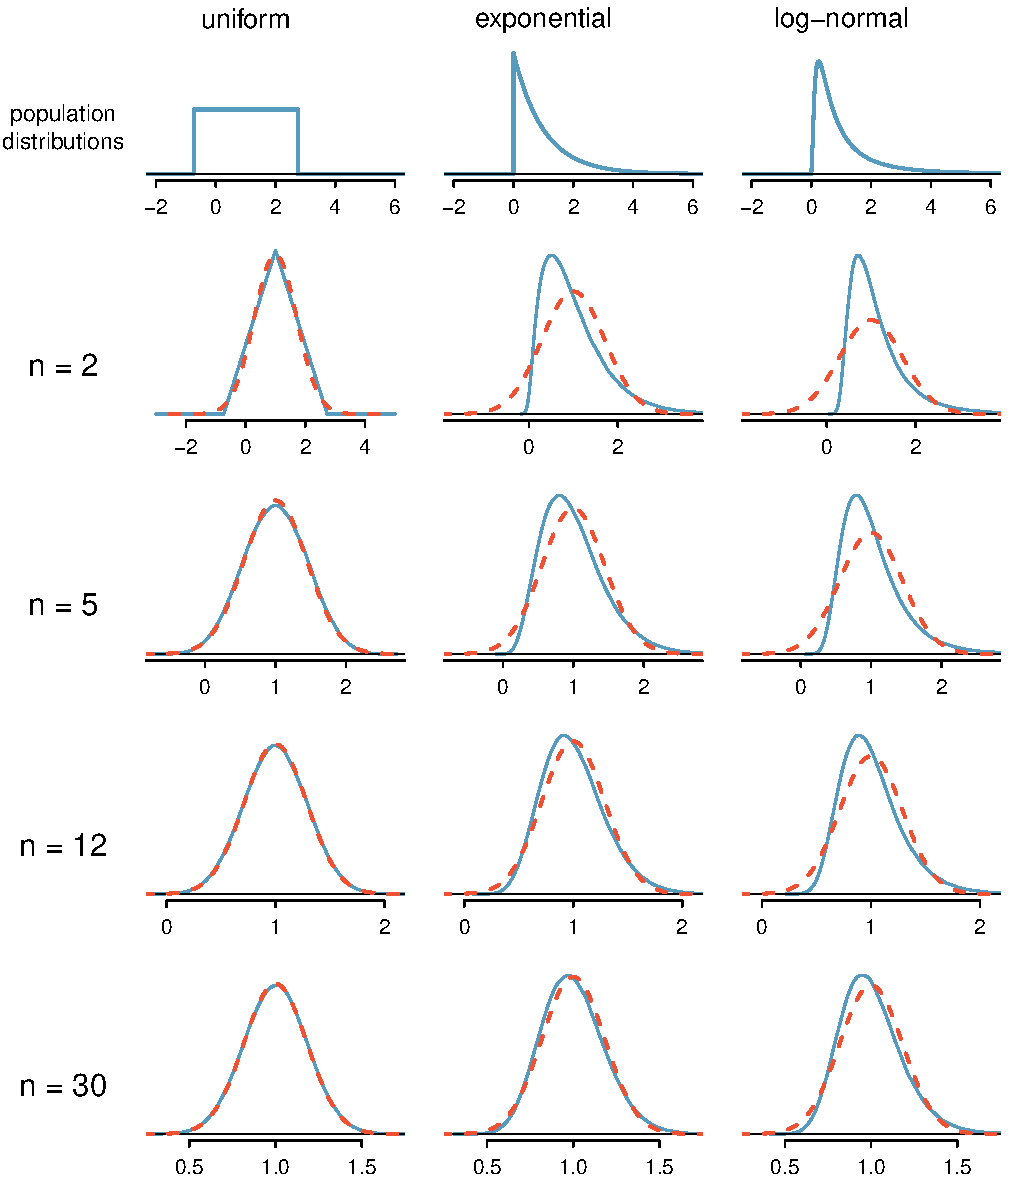
\includegraphics[width=\textwidth]{ch_inference_foundations_oi_biostat/figures/cltSimulations/cltSimulations}
   \caption{Sampling distributions for the mean at different sample sizes and for three different distributions. The dashed red lines show normal distributions.}
   \label{cltSimulations}
\end{figure}

The left panel in the $n=2$ row shows the theoretical sampling distribution of $\overline{x}$ if it a sample mean of two observations from the uniform distribution. The dashed line represents the closest approximation of the normal distribution. Similarly, the center and right panels of the $n=2$ row show the respective distributions of $\overline{x}$ for data from exponential and log-normal distributions.

\begin{exercise}
Examine the distributions in each row of Figure~\ref{cltSimulations}. What do you notice about the normal approximation for each sampling distribution as the sample size becomes larger?\footnote{The normal approximation becomes better as larger samples are used.}
\end{exercise}

\begin{example}{Would the normal approximation be good in all applications for a sample size of 30?}
Not necessarily. For example, the normal approximation for the log-normal example is questionable for a sample size of 30. Generally, the more skewed a population distribution or the more common the frequency of outliers, the larger the sample required to guarantee the distribution of the sample mean is nearly normal.
\end{example}

As discussed in Section~\ref{seOfTheMean}, the sample standard deviation, $s$, is often used  used as a substitute for the population standard deviation, $\sigma$, when computing the standard error. This estimate tends to be reasonable when $n\geq30$. Alternative approaches for smaller sample sizes are discussed in in Chapters~\ref{inferenceForNumericalData} and~\ref{inferenceForCategoricalData}.

%DH:  don't like this example.  Not biological, is only hypothetical and does not explain how the independence assumption is checked.  Does not provide practical guidance to a student, and should be replaced.

\begin{example}{Figure~\ref{pokerProfitsCanApplyNormalToSampMean} shows a histogram of 50  hypothetical observations --  winnings and losses from 50 consecutive days of a professional poker player. Can the normal approximation be applied to the sample mean, 90.69?}

\begin{itemize}
\setlength{\itemsep}{0mm}
\item[(1)] These are referred to as \term{time series data}, because the data arrived in a particular sequence. If the player wins on one day, it may influence how she plays the next. To make the assumption of independence we should perform careful checks on such data. While the supporting analysis is not shown, no evidence was found to indicate the observations are not independent.
\item[(2)] The sample size is 50, satisfying the sample size condition.
\item[(3)] There are two outliers, one very extreme, which suggests the data are very strongly skewed or very distant outliers may be common for this type of data. Outliers can play an important role and affect the distribution of the sample mean and the estimate of the standard error.
\end{itemize}
Since we should be skeptical of the independence of observations and the very extreme upper outlier poses a challenge, we should not use the normal model for the sample mean of these 50 observations. If we can obtain a much larger sample, perhaps several hundred observations, then the concerns about skew and outliers would no longer apply.
\end{example}

\begin{figure}[ht]
   \centering
   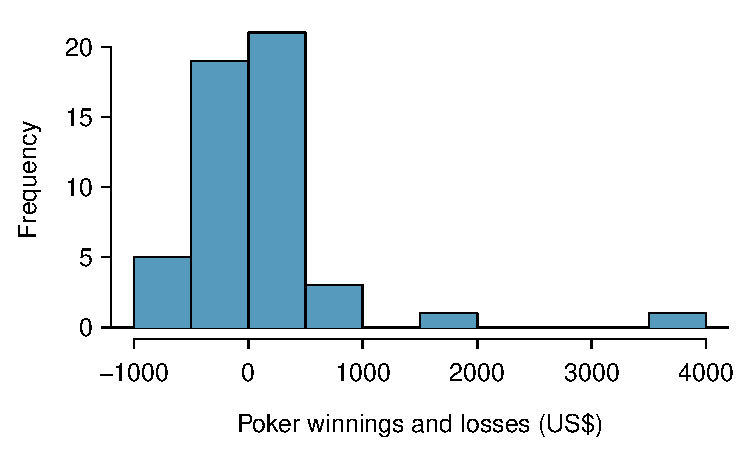
\includegraphics[height=58mm]{ch_inference_foundations_oi_biostat/figures/pokerProfitsCanApplyNormalToSampMean/pokerProfitsCanApplyNormalToSampMean}
   \caption{Sample distribution of poker winnings. These data include some very clear outliers. These are problematic when considering the normality of the sample mean. For example, outliers are often an indicator of very strong skew\index{skew!example: very strong}.}
   \label{pokerProfitsCanApplyNormalToSampMean}
\end{figure}

\begin{caution}
{Examine data structure when considering independence}
{Some data sets are collected in such a way that they have a natural underlying structure between observations, e.g. when observations occur consecutively. Be especially cautious about independence assumptions regarding such data sets.}
\end{caution}

\begin{caution}{Watch out for strong skew and outliers}
{Strong skew is often identified by the presence of clear outliers. If a data set has prominent outliers, or such observations are somewhat common for the type of data under study, then it is useful to collect a sample with many more than 30 observations if the normal model will be used for $\bar{x}$.}
\index{Central Limit Theorem|)}
\end{caution}

\index{skew!strongly skewed guideline}

\end{comment}

\section[Summary]{Summary}
\label{ch4Summary}

Confidence intervals and hypothesis testing are two of the central concepts in inference for a population based on a sample. The confidence interval shows a range of population parameter values consistent with the observed sample, and is often used to design additional studies. Hypothesis testing is a useful tool for evaluating the strength of the evidence against a working hypothesis according to a pre-specified standard for accepting or rejecting hypotheses.

The calculation of $p$-values and confidence intervals is relatively straightforward; given the necessary summary statistics, $\alpha$, and confidence coefficients, finding any $p$-value or confidence interval simply involves a set of formulaic steps. However, the more difficult parts of any inference problem are the steps that do not involve any calculations. Specifying appropriate null and alternative hypotheses for a test relies on an understanding of the problem context and the scientific setting of the investigation. Similarly, a choice about a confidence coefficient for an interval relies on judgment as to balancing precision against the chance of possible error. It is also not necessarily obvious when a significance level other than $\alpha = 0.05$ should be applied. These choices represent the largest distinction between a true statistics problem as compared to a purely mathematical exercise. 

Furthermore, in order to rely on the conclusions drawn from making inferences, it is necessary to consider factors such as study design, measurement quality, and the validity of any assumptions made. For example, is it valid to use the normal approximation to calculate $p$-values? In small to moderate sample sizes ($30 \leq n \leq 50$), it may not be clear that the normal model is accurate. It is even necessary to be cautious about the use and interpretation of the $p$-value. For example, an article published in \textit{Nature} about the mis-use of $p$-values references a published study that showed people who meet their spouses online are more likely to have marital satisfaction, with $p$-value less than 0.001. However, statistical significance does not measure the importance or practical relevance of a result; in this case, the change in happiness moved from 5.48 to 5.64 on a 7-point scale. A $p$-value reported without context or other evidence is uninformative and potentially deceptive.

%cite statistical_errors and asa_p_values

These nuanced issues cannot be adequately covered in any introduction to statistics. It is unrealistic to encourage students to use their own judgment with aspects of inference that even experienced investigators find challenging. At the same time, it would also be misleading to suggest that the choices are always clear-cut in practice. It seems best to offer some practical guidance for getting started:

\begin{itemize}
	\item The default choice of $\alpha$ is 0.05; similarly, the default confidence coefficient for a confidence interval is 95\%. 
	
	\item Unless it is clear from the context of a problem that change in only one direction from the null hypothesis is of interest, the alternative hypothesis should be two-sided.
	
	\item The use of a standard normal distribution to calculate $p$-values is reasonable for sample sizes of 30 or more if the distribution of data are not strongly skewed and there are no large outliers. If there is skew or a few large outliers, sample sizes of 50 or more are usually sufficient.
	
	\item Pay attention to the context of a problem, particularly when formulating hypotheses and drawing conclusions.
\end{itemize}

The next chapters will discuss methods of inference in specific settings, such as comparing two groups. These settings expand on the concepts discussed in this chapter and offer additional opportunities to practice calculating tests and intervals, reading problems for context, and checking underlying assumptions behind methods of inference.

\begin{comment}

%JV: DH draft

Confidence intervals and hypothesis tests are two of the central ideas and concepts in inference for a population based on a sample, and both will be used frequently in later chapters.  A confidence interval provides a plausible interval estimate for a population parameter along with a confidence coefficient, while a hypothesis test is a tool for making a qualitative yes/no decision about the parameter. Both have value -- the confidence interval shows a range of population parameter values consistent with the data and the width of the interval reflects both the confidence coefficient and the inherent uncertainty or randomness in the sample. It is often used to design additional studies.  Hypothesis testing is useful when policy decisions will be made about an intervention (a new drug, for instance) or an association (the association of genotype with a phenotype).  The pre-specified value of $\alpha$ is a reliable measure of the likelihood of rejecting a null hypothesis incorrectly.  Most progress in science is incremental and controlling the type 1 error probability $\alpha$ keeps the chance of a false positive acceptability low in the face of the inherent variability in human and biological measurements.

The calculation of tests and confidence intervals is relatively straightforward -- once the hypotheses, $\alpha$, and the confidence coefficient have been specified.  For most students, however, (and indeed may experienced investigators) the steps that do not rely on calculation are the more difficult part of the problem.  Specific null and alternative hypotheses and conclusions from a test are entirely context dependent -- driven by the scientific setting of the investigation.  The confidence coefficient reflects a study team's judgement on the balance of precision (the width of the interval) and chance of possible error (1 minus the confidence coefficient). The normal distribution used to calculate probabilities for the $t$ statistic is an approximation and in small to moderate sample sizes ($30 \leq n \leq 50$) it may not be clear that the normal model is adequate.  These choices, often based on judgement, may be the largest distinction between a statistics problem and a purely mathematical problem.

These nuanced issues cannot be adequately covered in any introduction to statistics. Urging students to use their judgement is not realistic (or fair) and prescribing choices of $\alpha$ and other aspects of inference may misleads student into thinking the choices are always clear. It seems best to offer some guidance on reasonable choices to get started:

\begin{itemize}
	
	\item Unless it is clear in the context of a problem that a specific direction of change from a null hypothesis is the one of interest, alternative hypotheses should be two-sided.
	
	\item In science, the usual choice for $\alpha$ is 0.05; that should be the default value unless otherwise specified in a problem.
	
	\item Similarly, the default value of the confidence coefficient for a confidence interval should 95\%, since it corresponds to a 5\% chance of error for the interval.
	
	\item The use of a standard normal distribution to calculate probabilities for a $t$-statistic is reasonable for sample sizes of 30 or more if the distribution of the data are not strongly skewed and there are no large outliers.  Later chapters will provide methods that can be used with small samples.
	
	\item Sample sizes of 50 or more are usually sufficient in the presence of skewing or a few large outliers.
		
\end{itemize}

The next chapters will cover methods of inference in specific scientific settings -- comparing two groups or fitting lines to data, for instance. These settings will provide opportunities to calculate tests and intervals, read problems for context and check some of the underlying assumptions.

\end{comment}



\end{spacing}
 


